%%%%%%%%%%%%%%%%%%%%%%%%%%%%% Thesis.tex %%%%%%%%%%%%%%%%%%%%%%%%%%%%%%%
%                                                                      %
%  ---------- Master of Science Dissertation template ----------       %
%                                                                      %
%  Template for the Master Thesis according to the regulations         %
%  published by the Academic Board (Direcção Académica) at IST.        %
%                                                                      %
%  For up-to-date guide, please refer to the offical website           %
%  http://da.tecnico.ulisboa.pt/dissertacao-de-mestrado/               %
%                                                                      %
%       Andre C. Marta                                                 %
%       Area Cientifica de Mecanica Aplicada e Aeroespacial            %
%       Departamento de Engenharia Mecanica                            %
%       Instituto Superior Tecnico                                     %
%       Av. Rovisco Pais                                               %
%       1049-001 Lisboa                                                %
%       Portugal                                                       %
%       Tel: +351 21 841 9469                                          %
%                        3469 (extension)                              %
%       Email: andre.marta@tecnico.ulisboa.pt                          %
%                                                                      %
%  Created:       Jan 20, 2011                                         %
%  Last Modified: Jul  2, 2015                                         %
%                                                                      %%%%%%%%%%%%%%%%%%%%%%%%%%%%%%%%%%%%%%%%%%%%%%%%%%%%%%%%%%%%%%%%%%%%%%%%
%  Revision history                                                    %
%  v1 - 2011/01/24 - original template                                 %
%  v2 - 2012/10/30 - new IST image and glossary support                %
%  v3 - 2013/12/10 - update according to 2012/13 official guide        %
%  v4 - 2014/02/28 - new default for bibliography style                %
%  v5 - 2014/05/07 - update according to 2013/14 official guide        %
%  v6 - 2015/07/02 - cover page format fixed,                          %
%                    contents page numbering fixed,                    %
%                    better language support,                          %
%                    enhanced examples of tables,                      %
%                    new option for appendix page numbering format,    %
%                    custom bibliography style                         %
%%%%%%%%%%%%%%%%%%%%%%%%%%%%%%%%%%%%%%%%%%%%%%%%%%%%%%%%%%%%%%%%%%%%%%%%
%                                                                      %
% To generate the PDF file, type "make" at the terminal prompt.        %
%                                                                      %
% The IST template LaTeX package was created by the author             %
% and it can be downloaded from:                                       %
% https://fenix.ist.utl.pt/homepage/ist31052/                          %
%                                                                      %
% The external packages can be downloaded from                         %
% the Comprehensive TeX Archive Network at http://www.ctan.org/        %
%                                                                      %
% List of LaTex symbols:                                               %
% http://www.ctan.org/tex-archive/info/symbols/comprehensive/          %
%                                                                      %
% Help with LaTex can be found at                                      %
% http://www.giss.nasa.gov/tools/latex/ltx-2.html                      %
% http://en.wikibooks.org/wiki/LaTeX                                   %
%%%%%%%%%%%%%%%%%%%%%%%%%%%%%%%%%%%%%%%%%%%%%%%%%%%%%%%%%%%%%%%%%%%%%%%%

%%%%%%%%%%%%%%%%%%%%%%%%%%%%%%%%%%%%%%%%%%%%%%%%%%%%%%%%%%%%%%%%%%%%%%%%
%     Preamble                                                         %
%%%%%%%%%%%%%%%%%%%%%%%%%%%%%%%%%%%%%%%%%%%%%%%%%%%%%%%%%%%%%%%%%%%%%%%%

% ----------------------------------------------------------------------
%  Set the document class
% ----------------------------------------------------------------------
\documentclass[12pt,a4paper,twoside]{report}

% ----------------------------------------------------------------------
% Define external packages, language, margins, fonts and new commands
% ----------------------------------------------------------------------
%%%%%%%%%%%%%%%%%%%%%%%%%%%%%%%%%%%%%%%%%%%%%%%%%%%%%%%%%%%%%%%%%%%%%%%%
%                                                                      %
%     File: Thesis_Preamble.tex                                        %
%     Tex Master: Thesis.tex                                           %
%                                                                      %
%     Author: Andre C. Marta                                           %
%     Last modified : 9 Apr 2015                                       %
%                                                                      %
%%%%%%%%%%%%%%%%%%%%%%%%%%%%%%%%%%%%%%%%%%%%%%%%%%%%%%%%%%%%%%%%%%%%%%%%

% ----------------------------------------------------------------------
% Define document language.
% ----------------------------------------------------------------------

% 'inputenc' package
%
% Accept different input encodings.
% http://www.ctan.org/tex-archive/macros/latex/base/
%
% > allows typing non-english text in LaTeX sources.
%
% ******************************* SELECT *******************************
% \usepackage[latin1]{inputenc} % <<<<< Windows
\usepackage[utf8]{inputenc}   % <<<<< Linux
% ******************************* SELECT *******************************


% 'babel' package
%
% Multilingual support for Plain TeX or LaTeX.
% http://www.ctan.org/tex-archive/macros/latex/required/babel/
%
% > sets the variable names according to the language selected
%
% ******************************* SELECT *******************************
%\usepackage[portuguese]{babel} % <<<<< Portuguese
\usepackage[english]{babel} % <<<<< English
% ******************************* SELECT *******************************


% List of LaTeX variable names: \abstractname, \appendixname, \bibname,
%   \chaptername, \contentsname, \listfigurename, \listtablename, ...)
% http://www.tex.ac.uk/cgi-bin/texfaq2html?label=fixnam
%
% Changing the words babel uses (uncomment and redefine as necessary...)
%
\newcommand{\acknowledgments}{@undefined} % new LaTeX variable name
%
% > English
%
\addto\captionsenglish{\renewcommand{\acknowledgments}{Acknowledgments}}
%\addto\captionsenglish{\renewcommand{\contentsname}{Contents}}
%\addto\captionsenglish{\renewcommand{\listtablename}{List of Tables}}
%\addto\captionsenglish{\renewcommand{\listfigurename}{List of Figures}}
%\addto\captionsenglish{\renewcommand{\nomname}{Nomenclature}}
%\addto\captionsenglish{\renewcommand{\glossaryname}{Glossary}}
%\addto\captionsenglish{\renewcommand{\acronymname}{List of Acronyms}}
%\addto\captionsenglish{\renewcommand{\bibname}{References}} % Bibliography
%\addto\captionsenglish{\renewcommand{\appendixname}{Appendix}}

% > Portuguese
%
\addto\captionsportuguese{\renewcommand{\acknowledgments}{Agradecimentos}}
%\addto\captionsportuguese{\renewcommand{\contentsname}{Conte\'{u}do}}
%\addto\captionsportuguese{\renewcommand{\listtablename}{Lista de Figuras}}
%\addto\captionsportuguese{\renewcommand{\listfigurename}{Lista de Tabelas}}
\addto\captionsportuguese{\renewcommand{\nomname}{Lista de S\'{i}mbolos}} % Nomenclatura
%\addto\captionsportuguese{\renewcommand{\glossary}{Gloss'{\a}rio}}
%\addto\captionsportuguese{\renewcommand{\acronymname}{Lista de Abrevia\c{c}\~{o}es}}
%\addto\captionsportuguese{\renewcommand{\bibname}{Refer\^{e}ncias}} % Bibliografia
%\addto\captionsportuguese{\renewcommand{\appendixname}{Anexo}} % Apendice


% ----------------------------------------------------------------------
% Define cover fields in both english and portuguese.
% ----------------------------------------------------------------------
%
\newcommand{\coverThesis}{@undefined} % new LaTeX variable name
\newcommand{\coverSupervisors}{@undefined} % new LaTeX variable name
\newcommand{\coverExaminationCommittee}{@undefined} % new LaTeX variable name
\newcommand{\coverChairperson}{@undefined} % new LaTeX variable name
\newcommand{\coverSupervisor}{@undefined} % new LaTeX variable name
\newcommand{\coverMemberCommittee}{@undefined} % new LaTeX variable name
% > English
\addto\captionsenglish{\renewcommand{\coverThesis}{Thesis to obtain the Master of Science Degree in}}
\addto\captionsenglish{\renewcommand{\coverSupervisors}{Supervisor(s)}}
\addto\captionsenglish{\renewcommand{\coverExaminationCommittee}{Examination Committee}}
\addto\captionsenglish{\renewcommand{\coverChairperson}{Chairperson}}
\addto\captionsenglish{\renewcommand{\coverSupervisor}{Supervisor}}
\addto\captionsenglish{\renewcommand{\coverMemberCommittee}{Member of the Committee}}
% > Portuguese
\addto\captionsportuguese{\renewcommand{\coverThesis}{Disserta\c{c}\~{a}o para obten\c{c}\~{a}o do Grau de Mestre em}}
\addto\captionsportuguese{\renewcommand{\coverSupervisors}{Orientador(es)}}
\addto\captionsportuguese{\renewcommand{\coverExaminationCommittee}{J\'{u}ri}}
\addto\captionsportuguese{\renewcommand{\coverChairperson}{Presidente}}
\addto\captionsportuguese{\renewcommand{\coverSupervisor}{Orientador}}
\addto\captionsportuguese{\renewcommand{\coverMemberCommittee}{Vogal}}


% ----------------------------------------------------------------------
% Define default and cover page fonts.
% ----------------------------------------------------------------------

% Use Arial font as default
%
\renewcommand{\rmdefault}{phv}
\renewcommand{\sfdefault}{phv}

% Define cover page fonts
%
\def\FontLb{\Huge} % Main Title
\def\FontMb{\LARGE} % Subtitle
\def\FontSn{\Large} % Candidate's Name


% ----------------------------------------------------------------------
% Define page margins and line spacing.
% ----------------------------------------------------------------------

% 'geometry' package
%
% Flexible and complete interface to document dimensions.
% http://www.ctan.org/tex-archive/macros/latex/contrib/geometry/
%
% > set the page margins (2.5cm minimum in every side, as per IST rules)
%
\usepackage{geometry}	
\geometry{verbose,tmargin=3cm,bmargin=3cm,lmargin=3cm,rmargin=3cm}

% 'setspace' package
%
% Set space between lines.
% http://www.ctan.org/tex-archive/macros/latex/contrib/setspace/
%
% > allow setting line spacing (line spacing of 1.5, as per IST rules)
%
\usepackage{setspace}
\renewcommand{\baselinestretch}{1.5}


% ----------------------------------------------------------------------
% Include external packages.
% Note that not all of these packages may be available on all system
% installations. If necessary, include the .sty files locally in
% the <jobname>.tex file directory.
% ----------------------------------------------------------------------

% 'graphicx' package
%
% Enhanced support for graphics.
% http://www.ctan.org/tex-archive/macros/latex/required/graphics/
%
% > extends arguments of the \includegraphics command
%
\usepackage{graphicx}
\graphicspath{{../Figures/}}


% 'color' package
%
% Colour control for LaTeX documents.
% http://www.ctan.org/tex-archive/macros/latex/required/graphics/
%
% > defines color macros: \color{<color name>}
%
%\usepackage{color}


% 'amsmath' package
%
% Mathematical enhancements for LaTeX.
% http://www.ctan.org/tex-archive/macros/latex/required/amslatex/
%
% > American Mathematical Society plain Tex macros
%
\usepackage{amsmath}  % AMS mathematical facilities for LaTeX.
\usepackage{amsthm}   % Typesetting theorems (AMS style).
\usepackage{amsfonts} % 


% 'wrapfig' package
%
% Produces figures which text can flow around.
% http://www.ctan.org/tex-archive/macros/latex/contrib/wrapfig/
%
% > wrap figures/tables in text (i.e., Di Vinci style)
%
% \usepackage{wrapfig}


% 'subfigure' package
%
% Deprecated: Figures divided into subfigures.
% http://www.ctan.org/tex-archive/obsolete/macros/latex/contrib/subfigure/
%
% > subcaptions for subfigures
%
\usepackage{subfigure}


% 'subfigmat' package
%
% Automates layout when using the subfigure package.
% http://www.ctan.org/tex-archive/macros/latex/contrib/subfigmat/
%
% > matrices of similar subfigures
%
\usepackage{subfigmat}


% 'url' package
%
% Verbatim with URL-sensitive line breaks.
% http://www.ctan.org/tex-archive/macros/latex/contrib/url/
%
% > URLs in BibTex
%
% \usepackage{url}


% 'varioref' package
%
% Intelligent page references.
% http://www.ctan.org/tex-archive/macros/latex/required/tools/
%
% > smart page, figure, table and equation referencing
%
%\usepackage{varioref}


% 'dcolumn' package
%
% Align on the decimal point of numbers in tabular columns.
% http://www.ctan.org/tex-archive/macros/latex/required/tools/
%
% > decimal-aligned tabular math columns
%
\usepackage{dcolumn}
\newcolumntype{d}{D{.}{.}{-1}} % column aligned by the point separator '.'
\newcolumntype{e}{D{E}{E}{-1}} % column aligned by the exponent 'E'


% '' package
%
% Reimplementation of and extensions to LaTeX verbatim.
% http://www.ctan.org/tex-archive/macros/latex/required/tools/
%
% > provides the verbatim environment (\begin{verbatim},\end{verbatim})
%   and a comment environment (\begin{comment},  \end{comment})
%
% \usepackage{verbatim}


% 'moreverb' package
%
% Extended verbatim.
% http://www.ctan.org/tex-archive/macros/latex/contrib/moreverb/
%
% > supports tab expansion and line numbering
%
% \usepackage{moreverb}



% 'nomencl' package
%
% Produce lists of symbols as in nomenclature.
% http://www.ctan.org/tex-archive/macros/latex/contrib/nomencl/
%
% The nomencl package makes use of the MakeIndex program
% in order to produce the nomenclature list.
%
% Nomenclature
% 1) On running the file through LATEX, the command \makenomenclature
%    in the preamble instructs it to create/open the nomenclature file
%    <jobname>.nlo corresponding to the LATEX file <jobname>.tex and
%    writes the information from the \nomenclature commands to this file.
% 2) The next step is to invoke MakeIndex in order to produce the
%    <jobname>.nls file. This can be achieved by making use of the
%    command: makeindex <jobname>.nlo -s nomencl.ist -o <jobname>.nls
% 3) The last step is to invoke LATEX on the <jobname>.tex file once
%    more. There, the \printnomenclature in the document will input the
%    <jobname>.nls file and process it according to the given options.
%
% http://www-h.eng.cam.ac.uk/help/tpl/textprocessing/nomencl.pdf
%
% Nomenclature (produces *.nlo *.nls files)
\usepackage{nomencl}
\makenomenclature
%
% Group variables according to their symbol type
%
\RequirePackage{ifthen} 
\ifthenelse{\equal{\languagename}{english}}%
    { % English
    \renewcommand{\nomgroup}[1]{%
      \ifthenelse{\equal{#1}{R}}{%
        \item[\textbf{Roman symbols}]}{%
        \ifthenelse{\equal{#1}{G}}{%
          \item[\textbf{Greek symbols}]}{%
          \ifthenelse{\equal{#1}{S}}{%
            \item[\textbf{Subscripts}]}{%
            \ifthenelse{\equal{#1}{T}}{%
              \item[\textbf{Superscripts}]}{}}}}}%
    }{% Portuguese
    \renewcommand{\nomgroup}[1]{%
      \ifthenelse{\equal{#1}{R}}{%
        \item[\textbf{Simbolos romanos}]}{%
        \ifthenelse{\equal{#1}{G}}{%
          \item[\textbf{Simbolos gregos}]}{%
          \ifthenelse{\equal{#1}{S}}{%
            \item[\textbf{Subscritos}]}{%
            \ifthenelse{\equal{#1}{T}}{%
              \item[\textbf{Sobrescritos}]}{}}}}}%
    }%


% 'glossary' package
%
% Create a glossary.
% http://www.ctan.org/tex-archive/macros/latex/contrib/glossary/
%
% Glossary (produces *.glo *.ist files)
\usepackage[number=none]{glossary}
% (remove blank line between groups)
\setglossary{gloskip={}}
% (redefine glossary style file)
%\renewcommand{\istfilename}{myGlossaryStyle.ist}
\makeglossary


% 'rotating' package
%
% Rotation tools, including rotated full-page floats.
% http://www.ctan.org/tex-archive/macros/latex/contrib/rotating/
%
% > show wide figures and tables in landscape format:
%   use \begin{sidewaystable} and \begin{sidewaysfigure}
%   instead of 'table' and 'figure', respectively.
%
\usepackage{rotating}


% 'hyperref' package
%
% Extensive support for hypertext in LaTeX.
% http://www.ctan.org/tex-archive/macros/latex/contrib/hyperref/
%
% > Extends the functionality of all the LATEX cross-referencing
%   commands (including the table of contents, bibliographies etc) to
%   produce \special commands which a driver can turn into hypertext
%   links; Also provides new commands to allow the user to write adhoc
%   hypertext links, including those to external documents and URLs.
%
\usepackage[pdftex]{hyperref} % enhance documents that are to be
                              % output as HTML and PDF
\hypersetup{colorlinks,       % color text of links and anchors,
                              % eliminates borders around links
%            linkcolor=red,    % color for normal internal links
            linkcolor=black,  % color for normal internal links
            anchorcolor=black,% color for anchor text
%            citecolor=green,  % color for bibliographical citations
            citecolor=black,  % color for bibliographical citations
%            filecolor=magenta,% color for URLs which open local files
            filecolor=black,  % color for URLs which open local files
%            menucolor=red,    % color for Acrobat menu items
            menucolor=black,  % color for Acrobat menu items
%            pagecolor=red,    % color for links to other pages
            pagecolor=black,  % color for links to other pages
%            urlcolor=cyan,    % color for linked URLs
            urlcolor=black,   % color for linked URLs
	          bookmarks=true,         % create PDF bookmarks
	          bookmarksopen=false,    % don't expand bookmarks
	          bookmarksnumbered=true, % number bookmarks
	          pdftitle={Thesis},
            pdfauthor={Andre C. Marta},
            pdfsubject={Thesis Title},
            pdfkeywords={Thesis Keywords},
            pdfstartview=FitV,
            pdfdisplaydoctitle=true}


% 'hypcap' package
%
% Adjusting the anchors of captions.
% http://www.ctan.org/tex-archive/macros/latex/contrib/oberdiek/
%
% > fixes the problem with hyperref, that links to floats points
%   below the caption and not at the beginning of the float.
%
\usepackage[figure,table]{hypcap}


% 'natbib' package
%
% Flexible bibliography support.
% http://www.ctan.org/tex-archive/macros/latex/contrib/natbib/
%
% > produce author-year style citations
%
% \citet  and \citep  for textual and parenthetical citations, respectively
% \citet* and \citep* that print the full author list, and not just the abbreviated one
% \citealt is the same as \citet but without parentheses. Similarly, \citealp is \citep without parentheses
% \citeauthor
% \citeyear
% \citeyearpar
%
% ******************************* SELECT *******************************
%\usepackage{natbib}          % <<<<< References in alphabetical list Correia, Silva, ...
\usepackage[numbers]{natbib} % <<<<< References in numbered list [1],[2],...
% ******************************* SELECT *******************************


% 'notoccite' package
%
% Prevent trouble from citations in table of contents, etc.
% http://ctan.org/pkg/notoccite
%
% > If you have \cite com­mands in \sec­tion-like com­mands, or in \cap­tion,
%   the ci­ta­tion will also ap­pear in the ta­ble of con­tents, or list of what­ever.
%   If you are also us­ing an un­srt-like bib­li­og­ra­phy style, these ci­ta­tions will
%   come at the very start of the bib­li­og­ra­phy, which is con­fus­ing. This pack­age
%   sup­presses the ef­fect.
%
\usepackage{notoccite}


% 'multirow' package
%
% Create tabular cells spanning multiple rows
% http://www.ctan.org/pkg/multirow
%
\usepackage{multirow}


% 'booktabs' package
%
% Publication quality tables in LaTeX
% http://www.ctan.org/pkg/booktabs
%
% > en­hance the qual­ity of ta­bles in LaTeX, pro­vid­ing ex­tra com­mands.
%
% \renewcommand{\arraystretch}{<ratio>} % space between rows
%
\usepackage{booktabs}
%\newcommand{\ra}[1]{\renewcommand{\arraystretch}{#1}}


% 'pdfpages' package
%
% Include PDF documents in LaTeX
% http://www.ctan.org/pkg/pdfpages
%
% > in­clu­sion of ex­ter­nal multi-page PDF doc­u­ments in LaTeX doc­u­ments.
%   Pages may be freely se­lected and sim­i­lar to psnup it is pos­si­ble to put
%   sev­eral log­i­cal pages onto each sheet of pa­per.
%
% \includepdf{filename.pdf}
% \includepdf[pages={4-9},nup=2x3,landscape=true]{filename.pdf}
%
\usepackage{pdfpages}
\definecolor{uered}{RGB}{158,27,50}
\definecolor{uegray}{RGB}{88,89,91}
\definecolor{ueblack}{RGB}{0,0,0}
\usepackage{emptypage}
\usepackage{titlesec}


% ----------------------------------------------------------------------
% Define new commands to assure consistent treatment throughout document
% ----------------------------------------------------------------------

\newcommand{\ud}{\mathrm{d}}                % total derivative
\newcommand{\degree}{\ensuremath{^\circ\,}} % degrees

% Abbreviations

\newcommand{\mcol}{\multicolumn}            % table format

\newcommand{\eqnref}[1]{(\ref{#1})}
\newcommand{\class}[1]{\texttt{#1}}
\newcommand{\package}[1]{\texttt{#1}}
\newcommand{\file}[1]{\texttt{#1}}
\newcommand{\BibTeX}{\textsc{Bib}\TeX}

% Typefaces ( example: {\bf Bold text here} )
%
% > pre-defined
%   \bf % bold face
%   \it % italic
%   \tt % typewriter
%
% > newly defined
\newcommand{\tr}[1]{{\ensuremath{\textrm{#1}}}}   % text roman
\newcommand{\tb}[1]{{\ensuremath{\textbf{#1}}}}   % text bold face
\newcommand{\ti}[1]{{\ensuremath{\textit{#1}}}}   % text italic
\newcommand{\mc}[1]{{\ensuremath{\mathcal{#1}}}}  % math calygraphy
\newcommand{\mco}[1]{{\ensuremath{\mathcalold{#1}}}}% math old calygraphy
\newcommand{\mr}[1]{{\ensuremath{\mathrm{#1}}}}   % math roman
\newcommand{\mb}[1]{{\ensuremath{\mathbf{#1}}}}   % math bold face
\newcommand{\bs}[1]{\ensuremath{\boldsymbol{#1}}} % math symbol
\def\bm#1{\mathchoice                             % math bold
  {\mbox{\boldmath$\displaystyle#1$}}%
  {\mbox{\boldmath$#1$}}%
  {\mbox{\boldmath$\scriptstyle#1$}}%
  {\mbox{\boldmath$\scriptscriptstyle#1$}}}
\newcommand{\boldcal}[1]{{\ensuremath{\boldsymbol{\mathcal{#1}}}}}% math bold calygraphy

\titleformat{\chapter}[display]
  {\normalfont\bfseries\color{uegray}}
  {\fontsize{256}{256}\selectfont\thechapter}{0pt}
  {\fontsize{32}{32}\selectfont}
\titlespacing*{\chapter}{0pt}{-50pt}{40pt}

\titleformat{\section}
  {\normalfont\Large\bfseries}{\thesection}{1em}{}


%\usepackage[table]{xcolor}
\usepackage{tabularray}
\usepackage[table,xcdraw]{xcolor} % Adiciona o pacote xcolor para cores
\usepackage{booktabs} % Para linhas horizontais mais bonitas

\usepackage{pgf-pie} 

% Definição das cores oficiais
\definecolor{uered}{RGB}{158,27,50}
\definecolor{uegray}{RGB}{88,89,91}
\definecolor{ueblack}{RGB}{0,0,0} % file "Thesis_Preamble.tex"

%%%%%%%%%%%%%%%%%%%%%%%%%%%%%%%%%%%%%%%%%%%%%%%%%%%%%%%%%%%%%%%%%%%%%%%%
%     Begin Document                                                   %
%%%%%%%%%%%%%%%%%%%%%%%%%%%%%%%%%%%%%%%%%%%%%%%%%%%%%%%%%%%%%%%%%%%%%%%%
\begin{document}

% Set plain page style (no headers, footer with centered page number)
\pagestyle{plain}

% Set roman numbering (i,ii,...) before the start of chapters
\pagenumbering{roman}

% ----------------------------------------------------------------------
%  Cover page
% ----------------------------------------------------------------------
%%%%%%%%%%%%%%%%%%%%%%%%%%%%%%%%%%%%%%%%%%%%%%%%%%%%%%%%%%%%%%%%%%%%%%%%
%                                                                      %
%     File: Thesis_FrontCover.tex                                      %
%     Tex Master: Thesis.tex                                           %
%                                                                      %
%     Author: Andre C. Marta                                           %
%     Last modified :  2 Jul 2015                                      %
%                                                                      %
%%%%%%%%%%%%%%%%%%%%%%%%%%%%%%%%%%%%%%%%%%%%%%%%%%%%%%%%%%%%%%%%%%%%%%%%

\thispagestyle {empty}

% IST Logo - Signature A
% parameters: bb=llx lly urx ury (bounding box), width=h_length, height=v_length, angle=angle, scale=factor, clip=true/false, draft=true/false. 

\includegraphics[scale=0.5]{teseue-logo.pdf}
\vspace{0.5cm}
\textcolor{uegray}{\dotfill}

\begin{center}
%
% Figure (Image or plot)
\vspace{2.5cm}
% height = 50 mm
\includegraphics[height=50mm]{../Figures/Airbus_A350.jpg}

% Title, author and degree
\vspace{1.0cm}
{\FontLb Thesis Title} \\ % <<<<< EDIT TITLE
%\vspace{0.2cm}
%{\FontMn Subtitle (optional)} \\
%\vspace{1.9cm}
\vspace{2.6cm}
{\FontMb Candidate Full Name} \\ % <<<<< EDIT NAME
\vspace{2.0cm}
{\FontSn \coverThesis} \\
\vspace{0.3cm}
{\FontLb Aerospace Engineering} \\ % <<<<< EDIT COURSE
\vspace{1.0cm}
{\FontSn %
\begin{tabular}{ll}
 \coverSupervisors: & Prof. Full Name 1 \\ % <<<<< EDIT NAME
                    & Dr. Full Name 2    % <<<<< EDIT NAME
\end{tabular} } \\
\vspace{1.0cm}
{\FontMb \coverExaminationCommittee} \\
\vspace{0.3cm}
{\FontSn %
\begin{tabular}{c}
\coverChairperson:     Prof. Full Name          \\ % <<<<< EDIT NAME
\coverSupervisor:      Prof. Full Name 1 (or 2) \\ % <<<<< EDIT NAME
\coverMemberCommittee: Prof. Full Name 3           % <<<<< EDIT NAME
\end{tabular} } \\
\vspace{1.5cm}
{\FontMb Month Year} \\ % <<<<< EDIT DATE (corresponds to date of oral examination)
%

\vfill
{\FontSn Esta (e) dissertação/ relatório de estágio/ trabalho de projeto não inclui as críticas e sugestões feitas pelo Júri}
\end{center}

 % file "Thesis_FrontCover.tex"
\cleardoublepage

% ----------------------------------------------------------------------
% Dedication page (optional)
% ----------------------------------------------------------------------
%%%%%%%%%%%%%%%%%%%%%%%%%%%%%%%%%%%%%%%%%%%%%%%%%%%%%%%%%%%%%%%%%%%%%%%%
%                                                                      %
%     File: Thesis_Dedication.tex                                      %
%     Tex Master: Thesis.tex                                           %
%                                                                      %
%     Author: Andre C. Marta                                           %
%     Last modified :  2 Jul 2015                                      %
%                                                                      %
%%%%%%%%%%%%%%%%%%%%%%%%%%%%%%%%%%%%%%%%%%%%%%%%%%%%%%%%%%%%%%%%%%%%%%%%

\null\vskip5cm%
\begin{flushright}
     Dedicated to someone special...
\end{flushright}
\vfill\newpage

 % file "Thesis_Dedication.tex"
\cleardoublepage

% ----------------------------------------------------------------------
%  Acknowledgments (optional)
% ----------------------------------------------------------------------
%%%%%%%%%%%%%%%%%%%%%%%%%%%%%%%%%%%%%%%%%%%%%%%%%%%%%%%%%%%%%%%%%%%%%%%%
%                                                                      %
%     File: Thesis_Acknowledgments.tex                                 %
%     Tex Master: Thesis.tex                                           %
%                                                                      %
%     Author: Andre C. Marta                                           %
%     Last modified :  2 Jul 2015                                      %
%                                                                      %
%%%%%%%%%%%%%%%%%%%%%%%%%%%%%%%%%%%%%%%%%%%%%%%%%%%%%%%%%%%%%%%%%%%%%%%%

\section*{\acknowledgments}

% Add entry in the table of contents as section
\addcontentsline{toc}{section}{\acknowledgments}

A few words about the university, financial support, research advisor, dissertation readers, faculty or other professors, lab mates, other friends and family...

 % file "Thesis_Acknowledgements.tex"
\cleardoublepage

% ----------------------------------------------------------------------
%  Abstract (both in English and Portuguese)
% ----------------------------------------------------------------------
%%%%%%%%%%%%%%%%%%%%%%%%%%%%%%%%%%%%%%%%%%%%%%%%%%%%%%%%%%%%%%%%%%%%%%%%
%                                                                      %
%     File: Thesis_Resumo.tex                                          %
%     Tex Master: Thesis.tex                                           %
%                                                                      %
%     Author: Andre C. Marta                                           %
%     Last modified :  2 Jul 2015                                      %
%                                                                      %
%%%%%%%%%%%%%%%%%%%%%%%%%%%%%%%%%%%%%%%%%%%%%%%%%%%%%%%%%%%%%%%%%%%%%%%%

\section*{Resumo}

% Add entry in the table of contents as section
\addcontentsline{toc}{section}{Resumo}

Inserir o resumo em Português aqui com o máximo de 150 palavras e acompanhado de até cinco palavras-chave...

vfill

\textbf{\Large Palavras-chave:} palavra-chave1, palavra-chave2

   % file "Thesis_Resumo.tex"
\cleardoublepage

%%%%%%%%%%%%%%%%%%%%%%%%%%%%%%%%%%%%%%%%%%%%%%%%%%%%%%%%%%%%%%%%%%%%%%%%
%                                                                      %
%     File: Thesis_Abstract.tex                                        %
%     Tex Master: Thesis.tex                                           %
%                                                                      %
%     Author: Andre C. Marta                                           %
%     Last modified :  2 Jul 2015                                      %
%                                                                      %
%%%%%%%%%%%%%%%%%%%%%%%%%%%%%%%%%%%%%%%%%%%%%%%%%%%%%%%%%%%%%%%%%%%%%%%%

\section*{Abstract}

% Add entry in the table of contents as section
\addcontentsline{toc}{section}{Abstract}

Insert your abstract here with a maximum of 150 words, followed by up to five keywords...

vfill

\textbf{\Large Keywords:} keyword1, keyword2

 % file "Thesis_Abstract.tex"
\cleardoublepage

% ----------------------------------------------------------------------
%  Table of contents, list of tables, list of figures and nomenclature
% ----------------------------------------------------------------------

% Table of contents
%
\tableofcontents
\cleardoublepage 

% List of tables
%
% Add entry in the table of contents as section
\phantomsection
\addcontentsline{toc}{section}{\listtablename}
% Generate list
\listoftables
\cleardoublepage 

% List of figures
%
% Add entry in the table of contents as section
\phantomsection
\addcontentsline{toc}{section}{\listfigurename}
% Generate list
\listoffigures
\cleardoublepage 

\chapter*{List of Acronyms}
\addcontentsline{toc}{chapter}{List of Acronyms}
\markboth{List of Acronyms}{List of Acronyms}

\begin{longtable}{ll}
\textbf{CFD} & Computational Fluid Dynamics \\
\textbf{CSM} & Computational Structural Mechanics \\
\textbf{MDO} & Multi-Disciplinar Optimization \\
\end{longtable}

 % file "Thesis_Acronyms.tex"
\cleardoublepage

% Nomenclature
%
% entries of nomenclature list
%%%%%%%%%%%%%%%%%%%%%%%%%%%%%%%%%%%%%%%%%%%%%%%%%%%%%%%%%%%%%%%%%%%%%%%%
%                                                                      %
%     File: Thesis_Nomenclature.tex                                    %
%     Tex Master: Thesis.tex                                           %
%                                                                      %
%     Author: Andre C. Marta                                           %
%     Last modified : 21 Jan 2011                                      %
%                                                                      %
%%%%%%%%%%%%%%%%%%%%%%%%%%%%%%%%%%%%%%%%%%%%%%%%%%%%%%%%%%%%%%%%%%%%%%%%
%
% The definitions can be placed anywhere in the document body
% and their order is sorted by <symbol> automatically when
% calling makeindex in the makefile
%
% The \glossary command has the following syntax:
%
% \glossary{entry}
%
% The \nomenclature command has the following syntax:
%
% \nomenclature[<prefix>]{<symbol>}{<description>}
%
% where <prefix> is used for fine tuning the sort order,
% <symbol> is the symbol to be described, and <description> is
% the actual description.

% ----------------------------------------------------------------------
% Roman symbols [r]
\nomenclature[ru]{$\bf u$}{Velocity vector.}
\nomenclature[ru]{$u,v,w$}{Velocity Cartesian components.}
\nomenclature[rp]{$p$}{Pressure.}
\nomenclature[rC]{$C_D$}{Coefficient of drag.}
\nomenclature[rC]{$C_L$}{Coefficient of lift.}
\nomenclature[rC]{$C_M$}{Coefficient of moment.}

% ----------------------------------------------------------------------
% Greek symbols [g]
\nomenclature[g]{$\rho$}{Density.}
\nomenclature[g]{$\alpha$}{Angle of attack.}
\nomenclature[g]{$\beta$}{Angle of side-slip.}
\nomenclature[g]{$\mu$}{Molecular viscosity coefficient.}
\nomenclature[g]{$\kappa$}{Thermal conductivity coefficient.}

% ----------------------------------------------------------------------
% Subscripts [s]
\nomenclature[s]{$x,y,z$}{Cartesian components.}
\nomenclature[s]{$i,j,k$}{Computational indexes.}
\nomenclature[s]{$\infty$}{Free-stream condition.}
\nomenclature[s]{ref}{Reference condition.}
\nomenclature[s]{$n$}{Normal component.}

% ----------------------------------------------------------------------
% Supercripts [t]
\nomenclature[t]{T}{Transpose.}
\nomenclature[t]{*}{Adjoint.}

 % file "Thesis_Nomenclature.tex"
%
% Add entry in the table of contents as section
\phantomsection
\addcontentsline{toc}{section}{\nomname}
% Insert glossary/nomenclature section produced by MakeIndex
\printnomenclature
\cleardoublepage

% entries of glossary list
%%%%%%%%%%%%%%%%%%%%%%%%%%%%%%%%%%%%%%%%%%%%%%%%%%%%%%%%%%%%%%%%%%%%%%%%
%                                                                      %
%     File: Thesis_Glossary.tex                                        %
%     Tex Master: Thesis.tex                                           %
%                                                                      %
%     Author: Andre C. Marta                                           %
%     Last modified : 30 Oct 2012                                      %
%                                                                      %
%%%%%%%%%%%%%%%%%%%%%%%%%%%%%%%%%%%%%%%%%%%%%%%%%%%%%%%%%%%%%%%%%%%%%%%%
%
% The definitions can be placed anywhere in the document body
% and their order is sorted by <symbol> automatically when
% calling makeindex in the makefile
%
% The \glossary command has the following syntax:
%
% \glossary{entry}
%
% The \nomenclature command has the following syntax:
%
% \nomenclature[<prefix>]{<symbol>}{<description>}
%
% where <prefix> is used for fine tuning the sort order,
% <symbol> is the symbol to be described, and <description> is
% the actual description.

% ----------------------------------------------------------------------

\glossary{name={\textbf{MDO}},description={Multi-Disciplinar Optimization is an engineering technique that uses optimization methods to solve design problems incorporating two or more disciplines.}}

\glossary{name={\textbf{CFD}},description={Computational Fluid Dynamics is a branch of fluid mechanics that uses numerical methods and algorithms to solve problems that involve fluid flows.}}

\glossary{name={\textbf{CSM}},description={Computational Structural Mechanics is a branch of structure mechanics that uses numerical methods and algorithms to perform the analysis of structures and its components.}}

 % file "Thesis_Glossary.tex"

% Add entry in the table of contents as section
\phantomsection
\addcontentsline{toc}{section}{\glossaryname}
% Insert glossary section produced by MakeIndex
\printglossary
\cleardoublepage

% Set arabic numbering (1,2,...) after preface
%
\setcounter{page}{1}
\pagenumbering{arabic}

% ----------------------------------------------------------------------
%  Chapters
% ----------------------------------------------------------------------

%%%%%%%%%%%%%%%%%%%%%%%%%%%%%%%%%%%%%%%%%%%%%%%%%%%%%%%%%%%%%%%%%%%%%%%%
%                                                                      %
%     File: Thesis_Introduction.tex                                    %
%     Tex Master: Thesis.tex                                           %
%                                                                      %
%     Author: Andre C. Marta                                           %
%     Last modified :  2 Jul 2015                                      %
%                                                                      %
%%%%%%%%%%%%%%%%%%%%%%%%%%%%%%%%%%%%%%%%%%%%%%%%%%%%%%%%%%%%%%%%%%%%%%%%

\chapter{Introduction}
\label{chapter:introduction}

O presente relatório foi desenvolvido no âmbito do estágio curricular do Mestrado Integrado em Medicina Veterinária da Universidade de Évora, realizado entre 2 de setembro e 28 de fevereiro de 2025 no OneVet- Hospital Veterinário do Porto (HVP), sob orientação interna da Doutora Teresa Oliveira e orientação externa da Dra. Nina Rodrigues.

Este relatório encontra-se dividido em duas componentes:
\begin{enumerate}
    \item A primeira componente consiste numa análise descritiva da casuística acompanhada pelo autor durante o período de estágio, organizada pelas áreas de medicina preventiva, clínica cirúrgica, clínica médica, incluindo ainda uma breve referência aos exames complementares de diagnóstico.
    \item A segunda parte é dedicada à monografia sobre o tema “Sialoadenose responsiva a fenobarbital em cães”, complementada pela descrição de um caso clínico acompanhado no decurso do estágio.
\end{enumerate}






 % file "Thesis_Introduction.tex"
\cleardoublepage

%%%%%%%%%%%%%%%%%%%%%%%%%%%%%%%%%%%%%%%%%%%%%%%%%%%%%%%%%%%%%%%%%%%%%%%%
%                                                                      %
%     File: Thesis_Background.tex                                      %
%     Tex Master: Thesis.tex                                           %
%                                                                      %
%     Author: Andre C. Marta                                           %
%     Last modified :  2 Jul 2015                                      %
%                                                                      %
%%%%%%%%%%%%%%%%%%%%%%%%%%%%%%%%%%%%%%%%%%%%%%%%%%%%%%%%%%%%%%%%%%%%%%%%

\chapter{Casuística}
\label{chapter:Casuistica}



\section{Descrição do local de estágio}


O OneVet-Hospital Veterinário do Porto, localizado na cidade do Porto, possui mais de 20 anos de experiência na área de Medicina Veterinária. A sua equipa está disponível 24 horas por dia, ao longo de todo o ano, capacitada para atender qualquer emergência ou intervenção cirúrgica com a maior celeridade. 

Este hospital conta com uma equipa multidisciplinar altamente qualificada em diversas áreas, sendo considerado uma referência em Cardiologia, Dermatologia, Oncologia, Ortopedia, Traumatologia e Oftalmologia. Dispõe ainda de uma vasta gama de meios complementares de diagnóstico, incluindo Ecografia, Ecocardiografia, Radiografia, Tomografia Computorizada, Fluoroscopia, Endoscopia e Ressonância Magnética.

A constante dedicação e especialização da equipa contribui significativamente para o reconhecimento do HVP como hospital de referência, resultando assim, numa elevada casuística.
Durante o período de estágio, o hospital mudou de instalações, o que permitiu melhorar as condições de trabalho e aprendizagem, bem como o bem-estar e conforto dos pacientes. 

O novo espaço apresenta uma receção comum, com zonas de espera separadas para cães e gatos, de forma a minimizar o stress. Dispões de seis consultórios (três para cães e três para gatos), equipados com difusores de feromonas e de uma sala dedicada a momentos mais delicados, como a eutanásia, garantindo a privacidade dos tutores.

O Hospital conta ainda uma área destinada a doenças infetocontagiosas, com separação entre cães e gatos, uma unidade de cuidados intensivos, quatro áreas de internamento (cães de grande porte, restantes cães, gatos e animais exóticos), sala para preparação cirúrgica e duas salas cirúrgicas devidamente equipadas. O serviço de Imagiologia inclui todos os meios referidos anteriormente, dispondo ainda de laboratório de análises clínicas, farmácia, sala de esterilização e uma sala de quimioterapia.

\section{Análise de Casuística}

A estrutura de estágio baseou-se numa rotação semanal pelas diversas áreas: “Internamento”, “Consultas”, “Oncologia”, “Cardiologia”,” Dermatologia”, “Medicina Interna” e “Cirurgia”. Em todos os serviços, foi promovida a participação ativa dos estagiários nos procedimentos clínicos, sempre sob supervisão de médicos e/ou enfermeiros.

Foram realizados turnos no Internamento, em horário variável (das 8h00 às 16h00 e das 13h00 às 21h00), no serviço de Consultas e Cardiologia (das 12h00 às 20h00), em Cirurgia (das 9h00 às 17h00) e em Oncologia, Medicina Interna e Dermatologia (das 9h00 às 17h00). Adicionalmente, efetuaram-se turnos noturnos semanais (das 20h00 às 8h00), durante os quais foi possível acompanhar consultas de urgência e respetivas abordagens.

Numa primeira fase, será apresentada uma análise estatística da casuística acompanhada pelo autor durante os seis meses de estágio. Esta análise baseia-se nos casos observados durante os turnos diurnos e noturnos dos diversos serviços do hospital, sempre acompanhado por médicos veterinários representativos das respetivas áreas.

É importante salientar que a casuística aqui descrita não reflete a totalidade dos casos hospitalares, mas apenas os efetivamente acompanhados pelo autor. Adicionalmente, muitos pacientes apresentavam patologias concomitantes, pelo que o número total de casos registados poderá não corresponder ao número real de animais acompanhados.

De forma a facilitar a análise, a casuística foi dividida em três áreas clínicas: a Medicina Preventiva, Clínica Médica e Clínica Cirúrgica que foram, por sua vez, sub-categorizadas para permitir uma melhor análise destas áreas:

\begin{enumerate}
    \item Medicina preventiva: vacinação, desparasitação e Identificação eletrónica.
    \item 	Clínica médica: Cardiologia,Hematologia, Dermatologia, Doenças Infeciosas e Parasitárias, Endocrinologia, Gastroenterologia e Glândulas Anexas, Teriogenologia, Nefrologia e Urologia, Neurologia, Oftalmologia, Oncologia, Traumatologia e Doenças Músculoesqueléticas, Otorrinolaringologia, Pneumologia e Toxicologia. 
    \item Clínica cirúrgica: Ortopedia, Neurocirurgia, Tecidos Moles, Odontologia e Outros Procedimentos.
\end{enumerate}

Os casos foram organizados através da utilização de tabelas que incluem a frequência absoluta por espécie (Fip), exclusivamente animais da espécie canina e felina, a frequência absoluta do procedimento ou patologia (Fi) e a frequência relativa em percentagem (Fr (\%)).

\section{Distribuição da Casuística por espécie animal}

A distribuição casuística abrange as espécies canina (\textit{Canis lupus familiaris}) e felina (\textit{Felis catus}). Ao longo do estágio, foram registados, pelo autor, um total de $n=565$ casos referentes a estas espécies. A espécie canina apresentou maior representatividade, com uma frequência absoluta de $n=339$, enquanto a espécie felina correspondeu a $n=226$. Em termos de frequência relativa(Fr), estes valores equivalem a 60.0\% e 40.0\%, respetivamente. Não foram incluídos animais pertencentes a espécies exóticas, dado que a Médica Veterinária responsável por esta área se encontrava ausente por motivo de baixa médica. 


\begin{figure}[h!]
  \centering
  \begin{tikzpicture}
    \pie[color={uered, uegray}]{60/Canídeo, 40/Felino}
  \end{tikzpicture}
  \caption{Frequência relativa em percentagem (Fr (\%)), das espécies contempladas na 
casuística (N=565)}
  \label{fig:circular}
\end{figure}


\section{Distribuição da Casuística por área clínica}

A distrbuição da casuística por área clínica, apresentada na tabela \ref{tab:t1} , compreende um total de $n=588$ casos observados, divididos pelas três principais áreas da clínica de animais de companhia: "Clínica Médica", "Clínica Cirúrgica" e "Medicina Preventiva". Verificando os dados, a área com maior representatividade foi a Clínica Médica, com uma frequência relativa de $84\%$, seguida da Clínica Cirúrgica, com  $10.2\%$ e, por último, a Medicina Preventiva, com uma Fr inferior ($5.8\%$). 
Conforme referido anteriormente, o número de animais observados é inferior ao número total de casos clínicos registados, devido, o que se justifica pela presença de doenças concomitantes e pela existência de situações que necessitaram de seguimento cirúrgico.

% \usepackage{tabularray}
\begin{table}[h!]
\centering
\begin{tblr}{
  width = \linewidth,
  colspec = {Q[300]Q[196]Q[183]Q[146]Q[104]},
  cells = {c},
  hlines,
  vlines,
}
\textbf{Área Clínica} & \textbf{Fip (Canina)} & \textbf{Fip (Felina)} & \textbf{Fi (Total)} & \textbf{Fr (\%)} \\
Clínica Médica        & 289                   & 205                   & 494                 & \textbf{84.0}    \\
Clínica Cirúrgica     & 38                    & 22                    & 60                  & \textbf{10.2}    \\
Medicina Preventiva   & 19                    & 15                    & 34                  & \textbf{5.8}     \\
\textbf{ Total }      & \textbf{346}          & \textbf{242}          & \textbf{588}        & \textbf{100}     
\end{tblr}
\caption{Distribuição da casuística pelas três principais áreas clínicas, por espécie (Fip), frequência absoluta (Fi) e frequência relativa (Fr(\%))} 
\label{tab:t1}
\end{table}

\subsection{Medicina Preventiva}

Como referido anteriormente, a área clínica Medicina Preventiva foi aquela em que se registou o menor número de casos. Uma das principais razões para esta menor casuística relaciona-se com o reduzido contacto do autor com esta área específica durante o período de estágio. O procedimento mais representado foi a vacinação com $n=17$ casos, correspondente a uma frequência relativa de ($50.0\%$), seguido da desparasitação com $n=13$ casos ($38.2\%$), e por último a identificação eletrónica com $n=4$ casos ($11.8\%$). 

% \usepackage{tabularray}
\begin{table}[h!]
\centering
\begin{tblr}{
  width = \linewidth,
  colspec = {Q[325]Q[190]Q[177]Q[140]Q[100]},
  cells = {c},
  hlines,
  vlines,
}
\textbf{Procedimentos}   & \textbf{Fip (Canina)} & \textbf{Fip (Felina)} & \textbf{Fi (Total)} & \textbf{Fr (\%)} \\
Vacinação                & 11                    & 6                     & 17                  & \textbf{50.0}    \\
Desparasitação           & 6                     & 7                     & 13                  & \textbf{38.2}    \\
Identificação eletrónica & 2                     & 2                     & 4                   & \textbf{11.8}    \\
\textbf{ Total }         & 19                    & 15                    & 34                  & \textbf{100}     
\end{tblr}
\caption{Distribuição da casuística de procedimentos observados na área clínica Medicina Preventiva, por espécie (Fip), frequência absoluta (Fi) e frequência relativa (Fr(\%))} 
\label{tab:t2}
\end{table}

\subsection{Clínica Médica}

A Clínica Médica representa a área clínica que apresentou maior casuística com um total de $n=494$ casos, correspondendo a uma frequência relativa de $84.0\%$. Trata-se de uma área que representa todas as doenças diagnosticadas durante os seis meses de estágio, subdivido em 15 áreas, posteriormente organizadas por ordem decrescente em relação ao número de casos.

Nesta área, o autor desenvolveu várias atividades desde a contenção de animais, colheita de sangue, estabelecimento de um acesso periférico, preparação de materiais para a realização de procedimentos, medição de pressões arteriais, preparação e administração de medicações, drenagem das cavidades torácica e abdominal, e até auxílio dos médicos e enfermeiros veterinários em diversas funções, como exames imagiológicos complementares, sendo eles a ultrassonografia, Raio X e Tomografia Computorizada.

Podemos então averiguar pela tabela \ref{tab:t3}, que a área com maior representatividade foi Gastroenterolia e Glândulas Anexas, com um total de $n=103$ casos ($Fr=20.8\%$), sendo, por esse motivo, a primeira a ser descrita no âmbito da Clínica Médica. Em extremo oposto, temos a Toxicologia, com apenas $n=5$ casos ($Fr=1.0\%$).

  % \usepackage{tabularray}
\begin{table}[h!]
\centering
\begin{tblr}{
  width = \linewidth,
  colspec = {Q[473]Q[142]Q[133]Q[106]Q[81]},
  cells = {c},
  hlines,
  vlines,
}
\textbf{Área Clínica}                       & \textbf{Fip (Canina)} & \textbf{Fip (Felina)} & \textbf{Fi (Total)} & \textbf{Fr (\%)} \\
Gastroenterologia e GA                      & 60                    & 43                    & 103                 & 20.8             \\
Nefrologia e Urologia                       & 13                    & 58                    & 71                  & 14.4             \\
Cardiologia                                 & 49                    & 20                    & 69                  & 14.0             \\
Oncologia                                   & 24                    & 29                    & 53                  & 10.7             \\
Doenças Infeciosas e Parasitárias           & 14                    & 24                    & 38                  & 7.7              \\
Endocrinologia                              & 15                    & 18                    & 33                  & 6.7              \\
Dermatologia                                & 22                    & 3                     & 25                  & 5.1              \\
Neurologia                                  & 23                    & 0                     & 23                  & 4.7              \\
Pneumologia                                 & 16                    & 5                     & 21                  & 4.3              \\
Otorrinolaringologia                        & 16                    & 2                     & 18                  & 3.6              \\
Oftalmologia                                & 11                    & 0                     & 11                  & 2.2              \\
Teriogenologia                              & 10                    & 0                     & 10                  & 2.0              \\
Traumatologia e Doenças Musculoesqueléticas & 6                     & 2                     & 8                   & 1.6              \\
Hematologia                                 & 5                     & 1                     & 6                   & 1.2              \\
Toxicologia                                 & 5                     & 0                     & 5                   & 1.0              \\
\textbf{TOTAL}                              & 289                   & 205                   & 494                 & 100              
\end{tblr}
\caption{Distribuição da casuística recolhida em Clínica Médica, por espécie (Fip), por frequência 
absoluta (Fi) e frequência relativa em percentagem (Fr(\%))} 
\label{tab:t3}
\end{table}
\subsubsection{Gastroenterologia e Glândulas anexas}

A especialidade de Gastroenterologia e GA dedica-se ao tratamento do trato digestivo, bem como de órgãos e glândulas anexas como o pâncreas, fígado, vesícula biliar e vias biliares. Esta foi a área, dentro da clínica médica, que mais casos registou. Foi responsável por $17.5\%$ da casuística recolhida durante o estágio curricular, correspondendo a $20.8\%$ de casos recolhidos em Clínica Médica.

De acordo com a tabela \ref{tab:t4} a afeção com maior representatividade foi a pancreatite, com  $n=21$ casos($Fr=20.4\%$) recolhidos. Em contraste, com uma frequência relativa de apenas $1.0\%$, doenças como cirrose hepática, colecistite e sialoadenose, foram as menos representadadas.

% \usepackage{tabularray}
\begin{table}[h!]
\centering
\begin{tblr}{
  width = \linewidth,
  colspec = {Q[477]Q[142]Q[133]Q[106]Q[81]},
  cells = {c},
  hlines,
  vlines,
}
\textbf{Gastroenterologia e gl. anexas}            & \textbf{Fip (Canina)} & \textbf{Fip (Felina)} & \textbf{Fi (Total)} & \textbf{Fr (\%)} \\
Pancreatite                                        & 6                     & 15                    & 21                  & \textbf{20.4}    \\
Doença
  inflamatória intestinal                   & 1                     & 13                    & 14                  & \textbf{13.6}    \\
Obstrução
  por corpo estranho gástrico/intestinal & 1                     & 3                     & 14                  & \textbf{13.6}    \\
Gastroenterite
  inespecífica                      & 7                     & 0                     & 7                   & \textbf{6.8}     \\
Enteropatia
  com perda de proteína                & 6                     & 0                     & 6                   & \textbf{5.8}     \\
Gastroenterite
  hemorrágica                       & 6                     & 0                     & 6                   & \textbf{5.8}     \\
Hepatite
  crónica                                 & 6                     & 0                     & 6                   & \textbf{5.8}     \\
Colangio-hepatite                                  & 1                     & 4                     & 5                   & \textbf{4.9}     \\
Megacólon
  idiopático                             & 4                     & 1                     & 5                   & \textbf{4.9}     \\
  Fecaloma                                           & 3                     & 0                     & 3                   & \textbf{2.9}     \\
Fístula perianal                                   & 3                     & 0                     & 3                   & \textbf{2.9}     \\
Lipidose
  hepática                                & 0                     & 3                     & 3                   & \textbf{2.9}     \\
Dilatação
  torção gástrica                        & 2                     & 0                     & 2                   & \textbf{1.9}     \\
Mucocelo                                           & 2                     & 0                     & 2                   & \textbf{1.9}     \\
Peritonite sética                                  & 0                     & 2                     & 2                   & \textbf{1.9}     \\
Triadite felina                                    & 0                     & 2                     & 2                   & \textbf{1.9}     \\
Cirrose
  hepática                                 & 1                     & 0                     & 1                   & \textbf{1.0}     \\
Colecistite                                        & 1                     & 0                     & 1                   & \textbf{1.0}     \\
Sialoadenose                                       & 1                     & 0                     & 1                   & \textbf{1.0}     \\
\textbf{TOTAL}                                     & 60                    & 43                    & 103                 & \textbf{100}     
\end{tblr}
\caption{Distribuição da casuística recolhida na especialidade Gastroenterologia e Glândulas Anexas, por 
espécie (Fip), por frequência absoluta (Fi), e frequência relativa em percentagem (Fr (\%)). } 
\label{tab:t4}
\end{table}

\subsubsection{Nefrologia e Urologia}

Estas duas especialidades- Nefrologia e Urologia- dedicam-se ao estudo e tratamento de doenças que afetam o sistema urinário, constituído pelos rins, ureteres, bexiga e uretra.
Esta área foi, a par da a Gastroenterologia e GA, uma das que apresentou maior casuística, com um total de $n=71$ casos registados, o que corresponde a uma frequência relativa de $14.4\%$ do total de casos da Clínica Médica. Destaca-se ainda por ter sido uma das áreas em que o número de casos em felídeos foi significativamente superior ao observado em canídeos.

Dado o elevado número de casos, a Nefrologia e urologia assumiram particular relevância para o autor, permitindo consolidar os conhecimentos previamente adquiridos ao longo da formação universitária, tanto no que respeita às abordagens clínicas e terapêuticas, como à realização e interpretação de exames complementares de diagnóstico.Entre estes, salientam-se a urinálise (tipos I e II), a urocultura, as análises bioquímicas e mensuração da densidade urinária.

De acordo com a tabela \ref{tab:t5}, conclui-se que a doença com maior representatividade, com larga margem, foi a doença renal crónica, contabilizando $n=37$ casos ($Fr=52.1\%$). Apenas duas doenças apresentaram maior incidência em cães do que em gatos: a hidronefrose e cistolitíase. Importa ainda referir que, dentro desta área, ocorreram situações que implicaram intervenção cirúrgica e que, por esse motivo, foram contabilizadas na secção de Clínica Cirúrgica, como os casos de ureterolitíase.

% \usepackage{tabularray}
\begin{table}[h!]
\centering
\begin{tblr}{
  width = \linewidth,
  colspec = {Q[408]Q[160]Q[146]Q[131]Q[92]},
  cells = {c},
  hlines,
  vlines,
}
\textbf{Nefrologia e urologia}     & \textbf{Fi (Canina)} & \textbf{Fi (Felina)} & \textbf{Fi (Total)} & \textbf{Fr (\%)} \\
Doença renal crónica (DRC)         & 7                    & 30                   & 37                  & \textbf{52.1}    \\
Cistite Idiopática Felina          & 0                    & 7                    & 7                   & \textbf{9.9}     \\
Cistolitiase                       & 4                    & 2                    & 6                   & \textbf{8.5}     \\
Ureterolitíase                     & 0                    & 6                    & 6                   & \textbf{8.5}     \\
Uretrolitíase                      & 0                    & 5                    & 5                   & \textbf{7.0}     \\
Infeção do trato urinário inferior & 0                    & 3                    & 3                   & \textbf{4.2}     \\
Doença renal Poliquística          & 0                    & 2                    & 2                   & \textbf{2.8}     \\
Hidronefrose                       & 2                    & 0                    & 2                   & \textbf{2.8}     \\
Lesão renal aguda (LRA)\textbf{}   & 0                    & 1                    & 1                   & \textbf{1.4}     \\
Megaureter                         & 0                    & 1                    & 1                   & \textbf{1.4}     \\
Ureter ectópico                    & 0                    & 1                    & 1                   & \textbf{1.4}     \\
\textbf{TOTAL}                     & 13                   & 58                   & 71                  & \textbf{100}     
\end{tblr}
\caption{ Distribuição da casuística recolhida na especialidade Nefrologia e Urologia, por espécie animal 
(Fip), por frequência absoluta (Fi), e frequência relativa em percentagem (Fr (\%))} 
\label{tab:t5}
\end{table}

\subsubsection{Cardiologia}

A especialidade de Cardiologia recai sobre as afeções do coração e sistema cardiovascular. Durante o seu estágio o aluno contactou com $n=69$ casos.

De acordo com tabela \ref{tab:t6}, dos 69 casos, as afeções mais observadas do foro cardiológico foram doença degenerativa da válvula mitral em cães e cardiomiopatia hipertrófica em gatos, com uma frequência relativa de $39.1\%$ e $17.4\%$, respetivamente.

% \usepackage{tabularray}
\begin{table}[h!]
\centering
\begin{tblr}{
  width = \linewidth,
  colspec = {Q[492]Q[133]Q[121]Q[108]Q[83]},
  cells = {c},
  hlines,
  vlines,
}
\textbf{Cardiologia}                         & \textbf{Fi (Canina)} & \textbf{Fi (Felina)} & \textbf{Fi (Total)} & \textbf{Fr (\%)} \\
Doença Degenerativa da Válvula Mitral (DDVM) & 27                   & 0                    & 27                  & \textbf{39.1}    \\
Cardiomiopatia hipertrófica                  & 0                    & 12                   & 12                  & \textbf{17.4}    \\
Cardiomiopatia dilatada                      & 9                    & 0                    & 9                   & \textbf{13.0}    \\
Bloqueio atrioventricular                    & 3                    & 0                    & 3                   & \textbf{4.3}     \\
Tromboembolismo aórtico                      & 0                    & 3                    & 3                   & \textbf{4.3}     \\
Estenose sub-aórtica                         & 3                    & 0                    & 3                   & \textbf{4.3}     \\
Falso tendão                                 & 3                    & 0                    & 3                   & \textbf{4.3}     \\
Movimento anterior sistólico (SAM)           & 0                    & 3                    & 3                   & \textbf{4.3}     \\
Persistência ducto arterioso                 & 2                    & 0                    & 2                   & \textbf{2.9}     \\
Estenose pulmonar                            & 0                    & 1                    & 1                   & \textbf{1.4}     \\
Insuficiência da válvula tricúspide          & 1                    & 0                    & 1                   & \textbf{1.4}     \\
Comunicação interventricular                 & 0                    & 1                    & 1                   & \textbf{1.4}     \\
Cor tiatriatum                               & 1                    & 0                    & 1                   & \textbf{1.4}     \\
\textbf{TOTAL}                               & 49                   & 20                   & 69                  & \textbf{100}     
\end{tblr}
\caption{Distribuição da casuística recolhida na especialidade de Cardiologia, por espécie animal (Fip), 
por frequência absoluta (Fi), e frequência relativa em percentagem (Fr (\%)) } 
\label{tab:t6}
\end{table}

\subsubsection{Oncologia}

A especialidade de Oncologia dedica-se ao estudo de todos os processos neoplásicos, desde o seu diagnóstico, tratamento e monitorização da evolução da doença. Nesta área foram observados um total de $n=53$casos, correspondendo a $Fr=10.7\%$ da casuística total observada na Clínica Médica.

De acordo com a tabela \ref{tab:t7}, podemos aferir que a afeção com maior representatividade é o linfoma alimentar, com $n=15$ casos recolhidos ($Fr=28.3\%$). De salientar que, nesta afeção, a prevalência foi observada unicamente em gatos. No entanto, no geral, houve maior representatividade de casos nos cães que nos gatos.

% \usepackage{tabularray}
\begin{table}[h!]
\centering
\begin{tblr}{
  width = \linewidth,
  colspec = {Q[469]Q[144]Q[135]Q[108]Q[83]},
  cells = {c},
  hlines,
  vlines,
}
\textbf{Oncologia}                             & \textbf{Fip (Canina)} & \textbf{Fip (Felina)} & \textbf{Fi (Total)} & \textbf{Fr (\%)} \\
Linfoma
  alimentar                            & 0                     & 15                    & 15                  & \textbf{28.3}    \\
Carcinoma
  das células escamosas              & 0                     & 7                     & 7                   & \textbf{13.2}    \\
Hemangiossarcoma
  esplénico                   & 6                     & 0                     & 6                   & \textbf{11.3}    \\
Mastocitoma
  cutâneo                          & 6                     & 0                     & 6                   & \textbf{11.3}    \\
Carcinoma
  mamário                            & 1                     & 4                     & 5                   & \textbf{9.4}     \\
Carcinoma
  das células de transição da bexiga & 2                     & 0                     & 2                   & \textbf{3.8}     \\
Linfoma
  mediastínico                         & 0                     & 2                     & 2                   & \textbf{3.8}     \\
Insulinoma                                     & 2                     & 0                     & 2                   & \textbf{3.8}     \\
Melanoma
  oral                                & 2                     & 0                     & 2                   & \textbf{3.8}     \\
Adenocarcinoma
  das glândulas hepatóides      & 1                     & 0                     & 1                   & \textbf{1.9}     \\
Adenoma
  esplénico                            & 1                     & 0                     & 1                   & \textbf{1.9}     \\
Adenoma
  hepático                             & 1                     & 0                     & 1                   & \textbf{1.9}     \\
Carcinoma pulmão                               & 1                     & 0                     & 1                   & \textbf{1.9}     \\
Hemangiossarcoma
  cardíaco                    & 1                     & 0                     & 1                   & \textbf{1.9}     \\
Hepatocarcinoma                                & 1                     & 0                     & 1                   & \textbf{1.9}     \\
Leucemia                                       & 1                     & 0                     & 1                   & \textbf{1.9}     \\
Linfoma
  gástrico                             & 1                     & 0                     & 1                   & \textbf{1.9}     \\
Linfoma ocular                                 & 0                     & 1                     & 1                   & \textbf{1.9}     \\
Melanocitoma
  palpebral                       & 1                     & 0                     & 1                   & \textbf{1.9}     \\
Osteossarcoma                                  & 1                     & 0                     & 1                   & \textbf{1.9}     \\
Timoma                                         & 1                     & 0                     & 1                   & \textbf{1.9}     \\
\textbf{TOTAL}                                 & 24                    & 29                    & 53                  & \textbf{ 100 }   
\end{tblr}
\caption{Distribuição da casuística recolhida na especialidade de Oncologia, por espécie animal (Fip), 
por frequência absoluta (Fi), e frequência relativa em percentagem (Fr (\%)) } 
\label{tab:t7}
\end{table}

\subsubsection{Doenças Infeciosas e Parasitárias}

A especialidade de Doenças Infeciosas e Parasitárias representou $7.7\%$ da totalidade da casuística acompanhada em clínica médica, correspondendo a um total de $n=38$ casos. 

Durante o estágio, o autor teve a oportunidade de realizar diversos testes rápidos de diagnóstico, nomeadamente para FIV, FELV, coronavírus e parvovírus, o que permitiu o desenvolvimento de competências práticas fundamentais.

 De acordo com a tabela \ref{tab:t8}, a afeção mais prevalente foi a parvovirose canina/panleucopénia felina, com $n=11$ casos ($Fr=28.9\%$).

Importa ainda referir que, ao longo do estágio, foram observados mais casos desta especialidade na espécie felina.

% \usepackage{tabularray}
\begin{table}
\centering
\begin{tblr}{
  width = \linewidth,
  colspec = {Q[465]Q[140]Q[131]Q[115]Q[85]},
  cells = {c},
  hlines,
  vlines,
}
\textbf{Doenças infeciosas e parasitárias} & \textbf{Fi (Canina)} & \textbf{Fi (Felina)} & \textbf{Fi (Total)} & \textbf{Fr (\%)} \\
Parvovirose canina/ Panleucopenia felina   & 5                    & 6                    & 11                  & \textbf{28.9}    \\
Leucemia felina (FELV)                     & 0                    & 5                    & 5                   & \textbf{13.2}    \\
Imunodeficiência viral felina (FIV)        & 0                    & 4                    & 4                   & \textbf{10.5}    \\
Leishmaniose                               & 4                    & 0                    & 4                   & \textbf{10.5}    \\
Peritonite infeciosa felina                & 0                    & 4                    & 4                   & \textbf{10.5}    \\
Calicivirose                               & 0                    & 3                    & 3                   & \textbf{~7.9}    \\
Leptospirose                               & 3                    & 0                    & 3                   & \textbf{7.9}     \\
Coriza                                     & 0                    & 2                    & 2                   & \textbf{5.3}     \\
Coronavírus                                & 1                    & 0                    & 1                   & \textbf{2.6}     \\
Dirofilariose                              & 1                    & 0                    & 1                   & \textbf{2.6}     \\
\textbf{TOTAL}                             & 14                   & 24                   & 38                  & \textbf{100}     
\end{tblr}
\caption{Distribuição da casuística recolhida na especialidade de Doenças infeciosas e parasitárias, por espécie animal (Fip), 
por frequência absoluta (Fi), e frequência relativa em percentagem (Fr (\%)) } 
\label{tab:t8}
\end{table}

\subsubsection{Endocrinologia}

Na especialidade Endocrinologia, área que se dedica ao estudo e tratamento de disfunções das glândulas endócrinas. Foram observados um total de $n=33$ casos ($Fr=6.7\%$). Durante o acompanhamento dos casos nesta especialidade, o estagiário assistiu à abordagem clínica dos médicos veterinários na realização do diagnóstico da doença endócrina e na apresentação das opções de tratamento e respetiva monitorização.
Durante o acompanhamento dos casos nesta especialidade, o estagiário assistiu à abordagem clínica dos médicos veterinários na realização do diagnóstico da doença endócrina e na apresentação das opções de tratamento e respetiva monitorização.

Através da tabela \ref{tab:t9}, verifica-se que a afeção diabetes mellitus foi a que obteve maior representatividade, com um total de $n=14$ casos. Estes catorze casos ficaram divididos em quatro casos da espécie canina e dez da espécie felina, obtendo uma $Fr=42.4\%$ dentro da especialidade. Sendo seguido pela afeção hipertiroidismo, que obteve também uma elevada representatividade com uma $Fr=24.2\%$. De salientar que foram recolhidos mais casos em gatos que cães nesta especialidade.

% \usepackage{tabularray}
\begin{table}
\centering
\begin{tblr}{
  width = \linewidth,
  colspec = {Q[475]Q[138]Q[127]Q[113]Q[85]},
  cells = {c},
  hlines,
  vlines,
}
\textbf{Endocrinologia}                   & \textbf{Fi (Canina)} & \textbf{Fi (Felina)} & \textbf{Fi (Total)} & \textbf{Fr (\%)} \\
Diabetes \textit{mellitus}                & 4                    & 10                   & 14                  & \textbf{42.4}    \\
Hipertiroidismo                           & 0                    & 8                    & 8                   & \textbf{24.2}    \\
Hiperadrenocorticismo hipófise-dependente & 4                    & 0                    & 4                   & \textbf{12.1}    \\
Hipoadrenocorticismo                      & 3                    & 0                    & 3                   & \textbf{9.1}     \\
Hipotiroidismo                            & 3                    & 0                    & 3                   & \textbf{9.1}     \\
Diabetes insipidus                        & 1                    & 0                    & 1                   & \textbf{3.0}     \\
\textbf{TOTAL}                            & 15                   & 18                   & 33                  & \textbf{100}     
\end{tblr}
\caption{Distribuição da casuística recolhida na especialidade de Endocrinologia, por espécie animal (Fip), 
por frequência absoluta (Fi), e frequência relativa em percentagem (Fr (\%)) } 
\label{tab:t9}
\end{table}

\subsubsection{Dermatologia}

A especialidade de Dermatologia dedica-se ao estudo, diagnóstico e tratamento das afeções relacionadas com a pele. Durante o estágio, foram registados um total de $n=25$ casos nesta área, sendo os cães os pacientes com maior representatividade, sobretudo devido ao elevado número de diagnósticos de dermatite atópica observados no hospital veterinário do porto.

A dermatite atópica/síndrome atópica felina foi a patologia mais frequentemente identificada, representando um total de $n=17$ casos ($Fr=68.0\%$), dos quais 15 ocorreram em cães. 

A experiência adquirida nesta especialidade permitiu o desenvolvimento e consolidação de competências práticas, nomeadamente na colheita de lesões cutâneas através de técnicas como a recolha de amostras por aposição, teste de fita cola e tricograma. Além disso, foi possível realizar a coloração adequada das amostras e proceder à sua interpretação microscópica, contribuindo significativamente para o diagnóstico das dermopatias.

% \usepackage{tabularray}
\begin{table}[h!]
\centering
\begin{tblr}{
  width = \linewidth,
  colspec = {Q[471]Q[140]Q[129]Q[113]Q[85]},
  cells = {c},
  hlines,
  vlines,
}
\textbf{Dermatologia }                     & \textbf{Fi (Canina)} & \textbf{Fi (Felina)} & \textbf{Fi (Total)} & \textbf{Fr (\%)} \\
Dermatite atópica/ Síndrome atópica felina & 15                   & 2                    & 17                  & \textbf{68.0}    \\
Alopécia X                                 & 3                    & 0                    & 3                   & \textbf{12.0}    \\
Pioderma superficial                       & 3                    & 0                    & 3                   & \textbf{12.0}    \\
Pênfigo foliáceo                           & 1                    & 1                    & 2                   & \textbf{8.0}     \\
\textbf{TOTAL}                             & 22                   & 3                    & 25                  & \textbf{100}     
\end{tblr}
\caption{Distribuição da casuística recolhida na especialidade de Dermatologia, por espécie animal (Fip), 
por frequência absoluta (Fi), e frequência relativa em percentagem (Fr (\%)) } 
\label{tab:t10}
\end{table}
\subsubsection{Neurologia}

A especialidade de Neurologia dedica-se ao estudo, diagnóstico e terapêutica de doenças do sistema nervoso, sendo necessário e de extrema importância saber realizar um exame neurológico pormenorizado e ter conhecimento da neuroanatomia, bem como saber interpretar exames imagiológicos, sendo de particular interesse nesta área, a tomografia computorizada e a radiografia. Não menos importante, saber fazer um bom exame ortopédico, é muitas vezes benéfico na diferenciação de lesões musculo-esqueléticas de lesões neurológicas.

A neurologia representou     dos casos registados em Clínica Médica e, observando a  tabela  , é possível aferir, que os cães representaram a totalidade dos casos ($n=22$)
Salienta-se que a hérnia discal obteve $n=8$ casos ($Fr=34.8\%$) da casuística na especialidade de Neurologia. 

Alguns casos tiveram seguimento para cirurgia, vindo a ser contabilizados na Clínica Cirúrgica, como é o caso das hérnias discais, onde foram posteriormente realizados procedimentos como hemilaminectomia e ventral slot.

% \usepackage{tabularray}
\begin{table}[h!]
\centering
\begin{tblr}{
  width = \linewidth,
  colspec = {Q[396]Q[162]Q[148]Q[133]Q[94]},
  cells = {c},
  hlines,
  vlines,
}
\textbf{Neurologia}            & \textbf{Fi (Canina)} & \textbf{Fi (Felina)} & \textbf{Fi (Total)} & \textbf{Fr (\%)} \\
Hérnia discal                  & 8                    & 0                    & 8                   & \textbf{34.8}    \\
Epilepsia idiopática           & 5                    & 0                    & 5                   & \textbf{21.7}    \\
Meningoencefalite              & 5                    & 0                    & 5                   & \textbf{21.7}    \\
Síndrome vestibular geriátrico & 2                    & 0                    & 2                   & \textbf{8.7}     \\
Discoespondilite               & 1                    & 0                    & 1                   & \textbf{4.3}     \\
Malformação chiari like        & 1                    & 0                    & 1                   & \textbf{4.3}     \\
Miastenia gravis               & 1                    & 0                    & 1                   & \textbf{4.3}     \\
\textbf{TOTAL}                 & 23                   & 0                    & 23                  & \textbf{100}     
\end{tblr}
\caption{Distribuição da casuística recolhida na especialidade de Neurologia, por espécie animal (Fip), 
por frequência absoluta (Fi), e frequência relativa em percentagem (Fr (\%)) } 
\label{tab:t11}
\end{table}

\subsubsection{Pneumologia}

A Pneumologia é a especialidade que se dedica ao estudo e tratamento de doenças pertencentes ao trato respiratório inferior, englobando a traqueia, brônquios, pulmões e pleura. Esta área foi responsável por 4.3\% da totalidade da casuística recolhida em Clínica Médica. 
Durante este estágio, foi possível ao estagiário assistir à realização e interpretação de radiografias torácicas, fundamentais para o diagnóstico das principais afeções respiratórias.
De acordo com a tabela \ref{tab:t12} , é possível aferir que a patologia com maior representatividade foi o colapso traqueal, com uma frequência absoluta de $n=6$ casos ($Fr=28.6\%$).
% \usepackage{tabularray}
\begin{table}[h!]
\centering
\begin{tblr}{
  width = \linewidth,
  colspec = {Q[462]Q[142]Q[133]Q[115]Q[85]},
  cells = {c},
  hlines,
  vlines,
}
\textbf{Pneumologia}                  & \textbf{Fi (Canina)} & \textbf{Fi (Felina)} & \textbf{Fi (Total)} & \textbf{Fr (\%)} \\
Colapso traqueal                      & 6                    & 0            & 6                   & \textbf{28.6}    \\
Pneumonia aspirativa                  & 4                    & 0           & 4                   & \textbf{19.0}    \\
Asma felina                           & 0                    & 3                    & 3                   & \textbf{14.3}    \\
Bronquite crónica                     & 3                    & 0                    & 3                   & \textbf{14.3}    \\
Contusão pulmonar secundária a trauma & 2                    & 0                    & 2                   & \textbf{9.5}     \\
Quilotórax idiopático                 & 0                    & 2                    & 2                   & \textbf{9.5}     \\
Hérnia Diafragmática                  & 1                    & 0                    & 1                   & \textbf{4.8}     \\
\textbf{TOTAL}                        & 16                   & 5                    & 21                  & \textbf{100}     
\end{tblr}
\caption{Distribuição da casuística recolhida na especialidade de Pneumologia, por espécie animal (Fip), 
por frequência absoluta (Fi), e frequência relativa em percentagem (Fr (\%)) } 
\label{tab:t12}
\end{table}

\subsubsection{Otorrinolaringologia}
A especialidade de Otorrinolaringologia dedica-se ao estudo, diagnóstico e tratamento das doenças que afetam os ouvidos, nariz, seios paranasais, faringe e laringe.

Esta área foi responsável por $3.6\%$ da totalidade da casuística registada em Clínica Médica. De acordo com os dados apresentados na tabela \ref{tab:t13}, verifica-se que todos os casos incidiram sobre a região do ouvido, com maior representatividade em cães do que em gatos. 

A afeção mais frequentemente diagnosticada foi a otite externa secundária a Malassezia spp, constituindo a principal causa de afeção otológica identificada durante o período de estágio.

% \usepackage{tabularray}
\begin{table}[h!]
\centering
\begin{tblr}{
  width = \linewidth,
  colspec = {Q[438]Q[150]Q[138]Q[123]Q[88]},
  cells = {c},
  hlines,
  vlines,
}
\textbf{Otorrinolaringologia}                       & \textbf{Fi (Canina)} & \textbf{Fi (Felina)} & \textbf{Fi (Total)} & \textbf{Fr (\%)} \\
Otite externa por \textbf{\textit{Malassezia spp.}} & 7                    & 0                    & 7                   & \textbf{38.9}    \\
Otite externa bacteriana                            & 6                    & 0                    & 6                   & \textbf{33.3}    \\
Oto-hematoma                                        & 2                    & 1                    & 3                   & \textbf{16.7}    \\
Otite média bacteriana                              & 1                    & 0                    & 1                   & \textbf{5.6}     \\
Otite média por pólipo nasofaríngeo                 & 0                    & 1                    & 1                   & \textbf{5.6}     \\
\textbf{TOTAL}                                      & 16                   & 2                    & 18                  & \textbf{100}     
\end{tblr}
\caption{Distribuição da casuística recolhida na especialidade de Otorrinolaringologia, por espécie animal (Fip), 
por frequência absoluta (Fi), e frequência relativa em percentagem (Fr (\%)) } 
\label{tab:t13}
\end{table}

\subsubsection{Oftalmologia}

A especialidade de Oftalmologia dedica-se ao estudo, diagnóstico e tratamento de doenças oculares. Trata-se de uma área que requer a realização de exames complementares específicos, tais como o teste de schirmer, a medição da pressão intraocular, o teste de fluoresceína, a biomicroscopia com lâmpada de fenda e a ultrassonografia ocular.

Durante o estágio, o autor acompanhou $n=11$ casos desta especialidade durante o período reservado a consultas, o que, em parte, justifica a menor casuística registada nesta área.

De acordo com a tabela \ref{tab:t14}, as doenças com maior representatividade foram a queratoconjuntivite seca e a úlcera superficial da córnea, ambas com uma frequência absoluta de dois casos ($Fr=18.2\%$)

Importa referir que todos os casos observados nesta área se restringiram à espécie canina.

% \usepackage{tabularray}
\begin{table}[h!]
\centering
\begin{tblr}{
  width = \linewidth,
  colspec = {Q[527]Q[121]Q[112]Q[100]Q[79]},
  cells = {c},
  hlines,
  vlines,
}
\textbf{Oftalmologia}                                             & \textbf{Fi (Canina)} & \textbf{Fi (Felina)} & \textbf{Fi (Total)} & \textbf{Fr (\%)} \\
Queratoconjuntivite seca                                          & 2                    & 0                    & 2                   & \textbf{18.2}    \\
Úlcera superficial da córnea                                      & 2                    & 0                    & 2                   & \textbf{18.2}    \\
Cataratas                                                         & 1                    & 0                    & 1                   & \textbf{9.1}     \\
Descemetocélio                                                    & 1                    & 0                    & 1                   & \textbf{9.1}     \\
Entrópio                                                          & 1                    & 0                    & 1                   & \textbf{9.1}     \\
Ectrópio                                                          & 1                    & 0                    & 1                   & \textbf{9.1}     \\
Prolapso da glândula da membrana nictitante (\textit{cherry eye}) & 1                    & 0                    & 1                   & \textbf{9.1}     \\
Síndrome de Degeneração Retiniana Adquirida Súbita                & 1                    & 0                    & 1                   & \textbf{9.1}     \\
Uveíte                                                            & 1                    & 0                    & 1                   & \textbf{9.1}     \\
\textbf{TOTAL}                                                    & 11                   & 0                    & 11                  & \textbf{100}     
\end{tblr}
\caption{Distribuição da casuística recolhida na especialidade de Oftalmologia, por espécie animal (Fip), 
por frequência absoluta (Fi), e frequência relativa em percentagem (Fr (\%)) } 
\label{tab:t14}
\end{table}

\subsubsection{Teriogenologia}

Teriogenologia é a área da medicina veterinária que se dedica ao estudo da fisiologia e das patologias do sistema reprodutivo animal. Foram recolhidos $n=10$ casos, sendo responsável por $2.0\%$ da totalidade da casuística registada em Clínica Médica.

De acordo com a Tabela \ref{tab:t15}, verifica-se que todos os casos se restringiram à espécie canina. 
A doença com maior representatividade foi a presença de quistos prostáticos, correspondendo a $40\%$ dos casos registados na área.
Tal como verificado noutras especialidades, os casos de piómetra implicaram seguimento cirúrgico, sendo posteriormente contabilizados na categoria de ovariohisterectomia, no âmbito da Clínica Cirúrgica.

% \usepackage{tabularray}
\begin{table}[h!]
\centering
\begin{tblr}{
  width = \linewidth,
  colspec = {Q[275]Q[194]Q[179]Q[160]Q[113]},
  cells = {c},
  hlines,
  vlines,
}
\textbf{Teriogenologia} & \textbf{Fi (Canina)} & \textbf{Fi (Felina)} & \textbf{Fi (Total)} & \textbf{Fr (\%)} \\
Quisto prostático       & 4                    & 0                    & 4                   & \textbf{40.0}    \\
Piómetra                & 3                    & 0                    & 3                   & \textbf{30.0}    \\
Parafimose              & 1                    & 0                    & 1                   & \textbf{10.0}    \\
Prostatite              & 1                    & 0                    & 1                   & \textbf{10.0}    \\
Vaginite                & 1                    & 0                    & 1                   & \textbf{10.0}    \\
\textbf{TOTAL}          & 10                   & 0                    & 10                  & \textbf{ 100 }   
\end{tblr}
\caption{Distribuição da casuística recolhida na especialidade de Teriogenologia, por espécie animal (Fip), 
por frequência absoluta (Fi), e frequência relativa em percentagem (Fr (\%)) } 
\label{tab:t15}
\end{table}

\subsubsection{Traumatologia e Doenças Musculoesqueléticas}

Esta área dedica-se ao estudo, diagnóstico e tratamento das afeções do aparelho locomotor. A abordagem eficaz destas patologias exige um sólido conhecimento anatómico, bem como competências práticas na realização de exames ortopédicos e neurológicos. Para além disso, assume particular relevância a capacidade de interpretação de exames de imagiologia, como a radiografia e a TC, fundamentais para uma avaliação completa das lesões musculoesqueléticas.

Durante o estágio, foram registados $n=8$ casos nesta especialidade, correspondendo a uma frequência relativa de $1.6\%$ da casuística total observada em Clínica Médica.

A doença com maior representatividade foi a rotura do ligamento cruzado cranial, com $n=4$ casos ($Fr=50.0\%$)

 \begin{table}[h!]
\centering
\begin{tblr}{
  width = \linewidth,
  colspec = {Q[502]Q[129]Q[119]Q[106]Q[81]},
  cells = {c},
  hlines,
  vlines,
}
\textbf{Traumatologia e Doenças Musculoesqueléticas} & \textbf{Fi (Canina)} & \textbf{Fi (Felina)} & \textbf{Fi (Total)} & \textbf{Fr (\%)} \\
Rotura do ligamento cruzado cranial                  & 4                    & 0                    & 4                   & \textbf{50.0}    \\
Fraturas ósseas                                      & 1                    & 2                    & 3                   & \textbf{37.5}    \\
Poliartrite
  imunomediada                           & 1                    & 0                    & 1                   & \textbf{12.5}    \\
\textbf{TOTAL}                                       & 6                    & 2                    & 8                   & \textbf{ 100 }             
\end{tblr}
\caption{Distribuição da casuística recolhida na especialidade de Traumatologia e Doenças Musculoesqueléticas, por espécie animal (Fip), 
por frequência absoluta (Fi), e frequência relativa em percentagem (Fr (\%)) } 
\label{tab:t16}
\end{table}

\subsubsection{Hematologia}

A especialidade de Hematologia dedica-se ao estudo, diagnóstico e tratamento de doenças do foro sanguíneo. No decurso do estágio, foram registados $n=6$ casos nesta área, correspondendo a uma $Fr= 1.2\%$ do total de casos observados em clínica médica.

De acordo com a tabela \ref{tab:t17}, verifica-se que a doença com maior representatividade foi a anemia hemolítica imunomediada.

% \usepackage{tabularray}
\begin{table}[h!]
\centering
\begin{tblr}{
  width = \linewidth,
  colspec = {Q[425]Q[154]Q[142]Q[127]Q[90]},
  cells = {c},
  hlines,
  vlines,
}
\textbf{Hematologia}           & \textbf{Fi (Canina)} & \textbf{Fi (Felina)} & \textbf{Fi (Total)} & \textbf{Fr (\%)} \\
Anemia hemolitica imunomediada & 4                    & 1                    & 5                   & \textbf{83.3}    \\
Trombocitopénia imunomediada   & 1                    & 0                    & 1                   & \textbf{16.7}    \\
\textbf{TOTAL}                 & 5                    & 1                    & 6                   & \textbf{100}     
\end{tblr}
\caption{Distribuição da casuística recolhida na especialidade de Hematologia, por espécie animal (Fip), 
por frequência absoluta (Fi), e frequência relativa em percentagem (Fr (\%)) } 
\label{tab:t17}
\end{table}

\subsubsection{Toxicologia}

A especialidade de Toxicologia dedica-se ao estudo, diagnóstico e tratamento dos sinais clínicos provocados resultantes da exposição a substâncias tóxicas, sejam elas ingeridas, inaladas, absorvidas ou inoculadas. 
Durante o estágio, a abordagem e monitorização clínica dos pacientes, bem como a realização de provas de coagulação, foram as principais atividades desenvolvidas no âmbito desta área, dada a relevância da avaliação da função hemostática em muitos quadros de intoxicação.

Esta especialidade apresentou um peso reduzido na casuística total da clínica médica, representando apenas $1.0\%$ dos casos registados.

 De acordo com a tabela \ref{tab:t18}, foram identifcados três tipos distintos de intoxicação, sendo a intoxicação por rodenticidas a mais prevalente, com $n=3$ casos ($Fr=60\%$).

 \begin{table}[h!]
\centering
\begin{tblr}{
  width = \linewidth,
  colspec = {Q[431]Q[152]Q[140]Q[125]Q[88]},
  cells = {c},
  hlines,
  vlines,
}
\textbf{Toxicologia}                & \textbf{Fi (Canina)} & \textbf{Fi (Felina)} & \textbf{Fi (Total)} & \textbf{Fr (\%)} \\
Rodenticidas                        & 3                    & 0                    & 3                   & \textbf{60.0}    \\
Intoxicação por lagarta do pinheiro & 1                    & 0                    & 1                   & \textbf{20.0}    \\
Paracetamol                         & 1                    & 0                    & 1                   & \textbf{20.0}    \\
\textbf{TOTAL}                      & 5                    & 0                    & 5                   & \textbf{100}             
\end{tblr}
\caption{Distribuição da casuística recolhida na especialidade de Toxicologia, por espécie animal (Fip), 
por frequência absoluta (Fi), e frequência relativa em percentagem (Fr (\%)) } 
\label{tab:t18}
\end{table}



\subsection{Clínica Cirúrgica}

Após a análise da casuística referente à Clínica Médica, constatou-se que a área da Clínica Cirúrgica apresentou um número inferior de casos, tendo sido registado um total de $n=60$ casos, o que corresponde a $10.2\%$ da casuística global observada.

A recolha da casuística foi realizada durante os turnos dedicados à cirurgia, nos quais o autor acompanhou os pacientes nas diferentes fases do procedimento cirúrgico: pré-operatório, intraoperatório e pós-operatório. 
Na fase pré-operatória, o autor colaborou com a equipa de anestesia na preparação dos pacientes, participando no cálculo e administração da medicação pré anestésica, na colocação de cateteres intravenosos, na administração de fluidoterapia, na tricotomia e respetiva assepsia da área a ser intervencionada, na entubação endotraqueal e na monitorização do paciente até à entrada no bloco operatório. 

Durante a fase intraoperatória, o autor desempenhou a função de ajudante de cirurgião, o que lhe permitiu uma observação privilegiada e direta do procedimento cirúrgico realizado em cada paciente. 

No período pós-operatório, a principal responsabilidade do estagiário consistiu na monitorização dos parâmetros vitais e recuperação dos pacientes, assegurando a sua estabilidade e resposta à intervenção.

Para facilitar a análise da casuística recolhida em Clínica Cirúrgica, os casos foram organizados em cinco categorias principais: cirurgia de tecidos moles, cirurgia odontológica, cirurgia ortopédica, neurocirurgia e outros procedimentos. 

De acordo com a tabela \ref{tab:t19}, que apresenta a distribuição da casuística cirúrgica, a cirurgia de tecidos moles destacou-se como a categoria com maior número de casos registados, representando $76.7\%$ da totalidade da casuística cirúrgica.

% \usepackage{tabularray}
\begin{table}
\centering
\begin{tblr}{
  width = \linewidth,
  colspec = {Q[346]Q[183]Q[171]Q[135]Q[96]},
  cells = {c},
  hlines,
  vlines,
}
\textbf{Clínica Cirúrgica} & \textbf{Fip (Canina)} & \textbf{Fip (Felina)} & \textbf{Fi (Total)} & \textbf{Fr (\%)} \\
Cirurgia de tecidos moles  & 27                    & 19                    & 46                  & \textbf{76.7}    \\
Cirurgia odontológica      & 9                     & 2                     & 11                  & \textbf{18.3}    \\
Neurocirurgia              & 2                     & 0                     & 2                   & \textbf{3.3}     \\
Cirurgia ortopédica        & 0                     & 1                     & 1                   & \textbf{1.7}     \\
\textbf{TOTAL}             & 38                    & 22                    & 60                  & \textbf{100}     
\end{tblr}
\caption{Distribuição da casuística recolhida em Clínica Cirúrgica, expressa em Frequência 
absoluta por espécie animal (Fip), Frequência absoluta (Fi) e Frequência relativa em percentagem (Fr\%).  } 
\label{tab:t19}
\end{table}
\subsubsection{Cirurgia de Tecidos Moles}

No total, foram recolhidos $n=46$ casos de cirurgia de tecidos moles. Como referido anteriormente, a cirurgia de tecidos moles destacou-se como a categoria com maior número de casos registados, representando $76.7\%$ da totalidade da casuística cirúrgica.
De acordo com a tabela \ref{tab:t20}, os procedimentos de esterilização e castração, são os que obtiveram uma maior representatividade. A ovariohisterectomia representou $17.4\%$ dos casos, enquanto que, a orquiectomia obteve uma frequência relativa de $21.7\%$.

% \usepackage{tabularray}
\begin{table}[h!]
\centering
\begin{tblr}{
  width = \linewidth,
  colspec = {Q[452]Q[150]Q[140]Q[112]Q[83]},
  cells = {c},
  hlines,
  vlines,
}
\textbf{Tecidos moles}                           & \textbf{Fip (Canina)} & \textbf{Fip (Felina)} & \textbf{Fi (Total)} & \textbf{Fr (\%)} \\
Orquiectomia                                     & 4                     & 6                     & 10                  & \textbf{21.7}    \\
Ovário-histerectomia (OVH )                      & 5                     & 3                     & 8                   & \textbf{17.4}    \\
Enterotomia                                      & 5                     & 1                     & 6                   & \textbf{13.0}    \\
Colocação de tubo de esofagostomia               & 0                     & 4                     & 4                   & \textbf{8.7}     \\
Colocação de\textit{ bypass} ureteral subcutâneo & 0                     & 3                     & 3                   & \textbf{6.5}     \\
Gastrotomia                                      & 3                     & 0                     & 3                   & \textbf{6.5}     \\
Mastectomia                                      & 2                     & 1                     & 3                   & \textbf{6.5}     \\
Nodulectomia                                     & 3                     & 0                     & 3                   & \textbf{6.5}     \\
Colocação pacemaker                              & 2                     & 0                     & 2                   & \textbf{4.3}     \\
Resolução de oto-hematoma                        & 2                     & 0                     & 2                   & \textbf{4.3}     \\
Biópsia pâncreas                                 & 1                     & 0                     & 1                   & \textbf{2.2}     \\
Enterectomia                                     & 0                     & 1                     & 1                   & \textbf{2.2}     \\
\textbf{TOTAL}                                   & 27                    & 19                    & 46                  & \textbf{100}     
\end{tblr}
\caption{Distribuição da casuística recolhida em Cirurgia de tecidos moles, expressa em Frequência 
absoluta por espécie animal (Fip), Frequência absoluta (Fi) e Frequência relativa em percentagem (Fr\%).  } 
\label{tab:t20}
\end{table}

\subsubsection{Cirurgia odontológica}

Nesta área foram recolhidos $n=11$ casos ($Fr=18.3\%$). De acordo com a tabela \ref{tab:t21}, podemos aferir que o procedimento odontológico com maior representatividade foi a destartarização e/ou extração dentária, com uma frequência absoluta de $n=10$ casos ($Fr=90.9\%$).

% \usepackage{tabularray}
\begin{table}[h!]
\centering
\begin{tblr}{
  width = \linewidth,
  colspec = {Q[454]Q[146]Q[135]Q[119]Q[87]},
  cells = {c},
  hlines,
  vlines,
}
\textbf{Odontologia}                   & \textbf{Fi (Canina)} & \textbf{Fi (Felina)} & \textbf{Fi (Total)} & \textbf{Fr (\%)} \\
Destartarização e/ou extração dentária & 8                    & 2                    & 10                  & \textbf{90.9}    \\
Remoção de melanoma oral               & 1                    & 0                    & 1                   & \textbf{9.1}     \\
\textbf{TOTAL}                         & 9                    & 2                    & 11                  & \textbf{100}     
\end{tblr}
\caption{Distribuição da casuística recolhida em Cirurgia odontológica, expressa em Frequência 
absoluta por espécie animal (Fip), Frequência absoluta (Fi) e Frequência relativa em percentagem (Fr\%).  } 
\label{tab:t21}
\end{table}

\subsubsection{Neurocirurgia}

Na área de neurocirurgia, foram recolhidos apenas dois casos ($Fr=3.3\%$).
De acordo com a tabela \ref{tab:t22}, é possível verificar que os procedimentos cirúrgicos realizados foram hemilaminectomia e ventral slot, para fim de correção de hérnias discais.

% \usepackage{tabularray}
\begin{table}[h!]
\centering
\begin{tblr}{
  width = \linewidth,
  colspec = {Q[281]Q[202]Q[188]Q[150]Q[106]},
  cells = {c},
  hlines,
  vlines,
}
\textbf{Neurocirurgia} & \textbf{Fip (Canina)} & \textbf{Fip (Felina)} & \textbf{Fi (Total)} & \textbf{Fr (\%)} \\
Hemilaminectomia       & 1                     & 0                     & 1                   & \textbf{50.0}    \\
Ventral slot           & 1                     & 0                     & 1                   & \textbf{50.0}    \\
\textbf{ TOTAL  }      & 2                     & 0                     & 2                   & \textbf{100}     
\end{tblr}
\caption{Distribuição da casuística recolhida em Neurocirurgia, expressa em Frequência 
absoluta por espécie animal (Fip), Frequência absoluta (Fi) e Frequência relativa em percentagem (Fr\%).  } 
\label{tab:t22}
\end{table}

\subsubsection{Cirurgia Ortopédica}

Ao longo dos 6 meses de estágio, o autor teve oportunidade de assistir e auxiliar apenas em uma cirurgia ortopédica, a qual representou uma frequência relativa de $1.7\%$ dos casos registados na clínica cirúrgica. 

Importa, no entanto, salientar que o Hospital Veterinário do Porto dispõe de todos os meios necessários para a realização de cirurgias ortopédicas, sendo esta limitação casuística apenas reflexo da ausência de casos desta natureza durante o período em que o autor esteve integrado na equipa cirúrgica.

\begin{table}[h!]
\centering
\begin{tblr}{
  width = \linewidth,
  colspec = {Q[488]Q[138]Q[129]Q[104]Q[81]},
  cells = {c},
  hlines,
  vlines,
}
\textbf{Cirurgia Ortopédica~}                        & \textbf{Fip (Canina)} & \textbf{Fip (Felina)} & \textbf{Fi (Total)} & \textbf{Fr (\%)} \\
Pins para resolução de múltiplas fraturas de dígitos & 0                     & 1                     & 1                   & \textbf{ 100 }   \\
\textbf{ TOTAL }                                     & 0                     & 1                     & 1                   & 100              
\end{tblr}
\caption{Distribuição da casuística recolhida em Cirurgia Ortopédica, expressa em Frequência 
absoluta por espécie animal (Fip), Frequência absoluta (Fi) e Frequência relativa em percentagem (Fr\%).  } 
\label{tab:t23}
\end{table}


\subsection{Procedimentos Médicos}

Na tabela \ref{tab:t24}, estão representados alguns procedimentos que o autor realizou, auxiliou ou assistiu e que, não podem ser contabilizados nas áreas mencionadas previamente.
Nesta área destaca-se o procedimento, cistocentese, com uma frequência absoluta de $n=77$ casos ($Fr=50.0\%$).

\begin{table}[h!]
\centering
\begin{tblr}{
  width = \linewidth,
  colspec = {Q[348]Q[175]Q[162]Q[142]Q[102]},
  cells = {c},
  hlines,
  vlines,
}
\textbf{Outros procedimentos} & \textbf{Fi (Canina)} & \textbf{Fi (Felina)} & \textbf{Fi (Total)} & \textbf{Fr (\%)} \\
Cistocentese                  & 31                   & 46                   & 77                  & \textbf{50.0}    \\
Toracocentese                 & 13                   & 11                   & 24                  & \textbf{15.6}    \\
Limpeza de feridas            & 11                   & 7                    & 18                  & \textbf{11.7}    \\
Transfusão sanguínea          & 5                    & 6                    & ~11                 & \textbf{7.1}     \\
Eutanásia                     & 6                    & 4                    & 10                  & \textbf{6.5}     \\
Quimioterapia                 & 4                    & 6                    & 10                  & \textbf{6.5}     \\
Abdominocentese               & 4                    & 0                    & 4~~                 & \textbf{2.6}     \\
\textbf{TOTAL}                & 74                   & 80                   & 154                 & \textbf{100}              
\end{tblr}
\caption{Distribuição da casuística recolhida em Procedimentos Médicos, expressa em Frequência 
absoluta por espécie animal (Fip), Frequência absoluta (Fi) e Frequência relativa em percentagem (Fr\%).  } 
\label{tab:t24}
\end{table}

\subsection{Exames Complementares de Diagnóstico}

Na tabela \ref{tab:t25}, podemos observar a casuística dos inúmeros exames complementares de diagnóstico em que o aluno participou. Como é possível aferir, os exames com maior representatividade foram, dentro da área de imagiologia, a ultrassonografia e radiografia.

\begin{table}[h!]
\centering
\begin{tblr}{
  width = \linewidth,
  colspec = {Q[121]Q[165]Q[229]Q[123]Q[113]Q[102]Q[79]},
  cells = {c},
  cell{1}{1} = {c=3}{0.515\linewidth},
  cell{2}{1} = {r=5}{},
  cell{2}{2} = {r=3}{},
  cell{5}{2} = {c=2}{0.394\linewidth},
  cell{6}{2} = {c=2}{0.394\linewidth},
  cell{7}{1} = {c=3}{0.515\linewidth},
  cell{8}{1} = {c=3}{0.515\linewidth},
  cell{9}{1} = {c=3}{0.515\linewidth},
  cell{10}{1} = {c=3}{0.515\linewidth},
  cell{11}{1} = {c=3}{0.515\linewidth},
  cell{12}{1} = {c=2,r=3}{0.286\linewidth},
  cell{15}{1} = {c=2,r=2}{0.286\linewidth},
  cell{17}{1} = {c=3}{0.515\linewidth},
  vlines,
  hline{1-2,7-12,15,17-18} = {-}{},
  hline{3-4,13-14,16} = {3-7}{},
  hline{5-6} = {2-7}{},
}
\textbf{Exames Complementares de Diagnóstico} &                  &                        & \textbf{Fi (Canina)} & \textbf{Fi (Felina)} & \textbf{Fi (Total)} & \textbf{Fr (\%)} \\
Imagiolo- gia                                  & Ultrasso- nografia & Abdominal              & 156                  & 187                  & 343                 & \textbf{52.3}    \\
                                             &                  & Ecocardiografia        & 44                   & 27                   & 71                  & \textbf{10.8}    \\
                                             &                  & Ocular                 & 2                    & 0                    & 2                   & \textbf{0.3}     \\
                                             & Radiografia      &                        & 41                   & 35                   & 76                  & \textbf{11.6}    \\
                                             & TC               &                        & 26                   & 5                    & 29                  & \textbf{4.4}     \\
Eletrocardiografia                           &                  &                        & 15                   & 12                   & 27                  & \textbf{4.1}     \\
Colheita de líquido Cefalorraquidiano        &                  &                        & 4                    & 2                    & 6                   & \textbf{0.9}     \\
Urinálise                                    &                  &                        & 16                   & 25                   & 41                  & \textbf{6.3}     \\
Teste de Schirmer                            &                  &                        & 2                    & 0                    & 2                   & \textbf{0.3}     \\
Teste de fluoresceína                        &                  &                        & 1                    & 0                    & 1                   & \textbf{0.2}     \\
Testes rápidos                               &                  & Parvovirus/ Coronavirus & 7                    & 5                    & 12                  & \textbf{1.8}     \\
                                             &                  & SNAP PLi               & 1                    & 3                    & 4                   & \textbf{0.6}     \\
                                             &                  & FIV/FELV               & 0                    & 4                    & 4                   & \textbf{0.6}     \\
Anatomo-histopatologia                       &                  & Citologia              & 11                   & 18                   & 29                  & \textbf{4.4}     \\
                                             &                  & Biópsia                & 4                    & 3                    & 7                   & \textbf{1.1}     \\
\textbf{TOTAL}
                             &                  &                        & 330                  & 326                  & 656                 & 100              
\end{tblr}
\caption{Distribuição da casuística recolhida em Exames Complementares de Diagnóstico, expressa em Frequência 
absoluta por espécie animal (Fip), Frequência absoluta (Fi) e Frequência relativa em percentagem (Fr\%).  } 
\label{tab:t25}
\end{table}





 % file "Thesis_Background.tex"
\cleardoublepage

%%%%%%%%%%%%%%%%%%%%%%%%%%%%%%%%%%%%%%%%%%%%%%%%%%%%%%%%%%%%%%%%%%%%%%%%
%                                                                      %
%     File: Thesis_Implementation.tex                                  %
%     Tex Master: Thesis.tex                                           %
%                                                                      %
%     Author: Andre C. Marta                                           %
%     Last modified :  2 Jul 2015                                      %
%                                                                      %
%%%%%%%%%%%%%%%%%%%%%%%%%%%%%%%%%%%%%%%%%%%%%%%%%%%%%%%%%%%%%%%%%%%%%%%%

\chapter{Implementation}
\label{chapter:implementation}

Insert your chapter material here...

%%%%%%%%%%%%%%%%%%%%%%%%%%%%%%%%%%%%%%%%%%%%%%%%%%%%%%%%%%%%%%%%%%%%%%%%
\section{Numerical Model}
\label{section:model}

Description of the numerical implementation of the models explained in Chapter~\ref{chapter:background}...


%%%%%%%%%%%%%%%%%%%%%%%%%%%%%%%%%%%%%%%%%%%%%%%%%%%%%%%%%%%%%%%%%%%%%%%%
\section{Verification and Validation}
\label{section:verification}

Basic test cases to compare the implemented model against other numerical tools (verification) and experimental data (validation)...

 % file "Thesis_Implementation.tex"
\cleardoublepage

%\input{Thesis_new_file} % add new .tex files for new chapters
% \cleardoublepage

%\input{Thesis_new_file} % add new .tex files for new chapters
% \cleardoublepage

%\input{Thesis_new_file} % add new .tex files for new chapters
% \cleardoublepage

%%%%%%%%%%%%%%%%%%%%%%%%%%%%%%%%%%%%%%%%%%%%%%%%%%%%%%%%%%%%%%%%%%%%%%%%
%                                                                      %
%     File: Thesis_Results.tex                                         %
%     Tex Master: Thesis.tex                                           %
%                                                                      %
%     Author: Andre C. Marta                                           %
%     Last modified :  2 Jul 2015                                      %
%                                                                      %
%%%%%%%%%%%%%%%%%%%%%%%%%%%%%%%%%%%%%%%%%%%%%%%%%%%%%%%%%%%%%%%%%%%%%%%%

\chapter{Results}
\label{chapter:results}

Insert your chapter material here... carlao lindao


%%%%%%%%%%%%%%%%%%%%%%%%%%%%%%%%%%%%%%%%%%%%%%%%%%%%%%%%%%%%%%%%%%%%%%%%
\section{Problem Description}
\label{section:problem}

Description of the baseline problem...


%%%%%%%%%%%%%%%%%%%%%%%%%%%%%%%%%%%%%%%%%%%%%%%%%%%%%%%%%%%%%%%%%%%%%%%%
\section{Baseline Solution}
\label{section:baseline}

Analysis of the baseline solution...


%%%%%%%%%%%%%%%%%%%%%%%%%%%%%%%%%%%%%%%%%%%%%%%%%%%%%%%%%%%%%%%%%%%%%%%%
\section{Enhanced Solution}
\label{section:enhanced}

Quest for the optimal solution...


% ----------------------------------------------------------------------
\subsection{Figures}
\label{subsection:figures}

Insert your section material and possibly a few figures...

Make sure all figures presented are referenced in the text!


% ----------------------------------------------------------------------
\subsubsection{Images}
\label{subsection:images}

\begin{figure}[!htb]
  \centering
  \includegraphics[width=0.25\textwidth]{Airbus_A350.jpg}
  \caption[Caption for figure in TOC.]{Caption for figure.}
  \label{fig:airbus1}
\end{figure}

\begin{figure}[!htb]
  \begin{subfigmatrix}{2}
    \subfigure[Airbus A320]{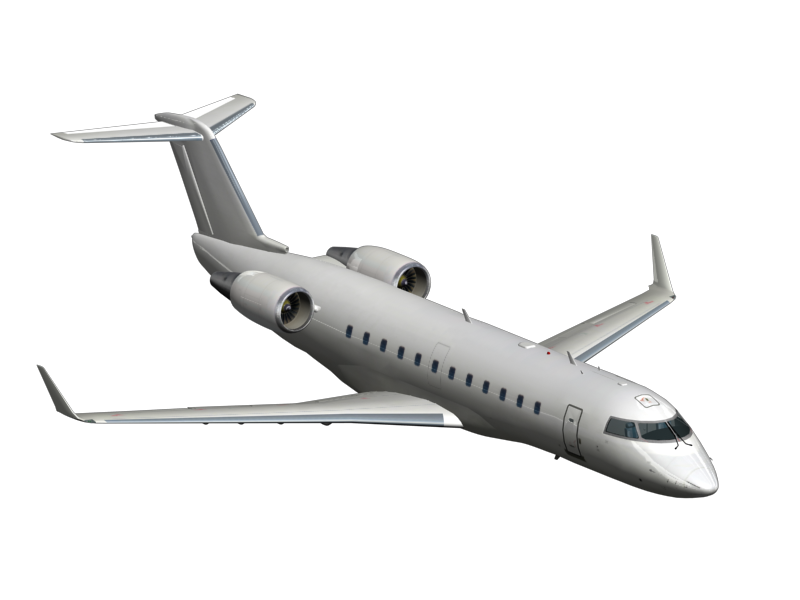
\includegraphics[width=\linewidth]{Bombardier_CRJ200}}
    \subfigure[Bombardier CRJ200]{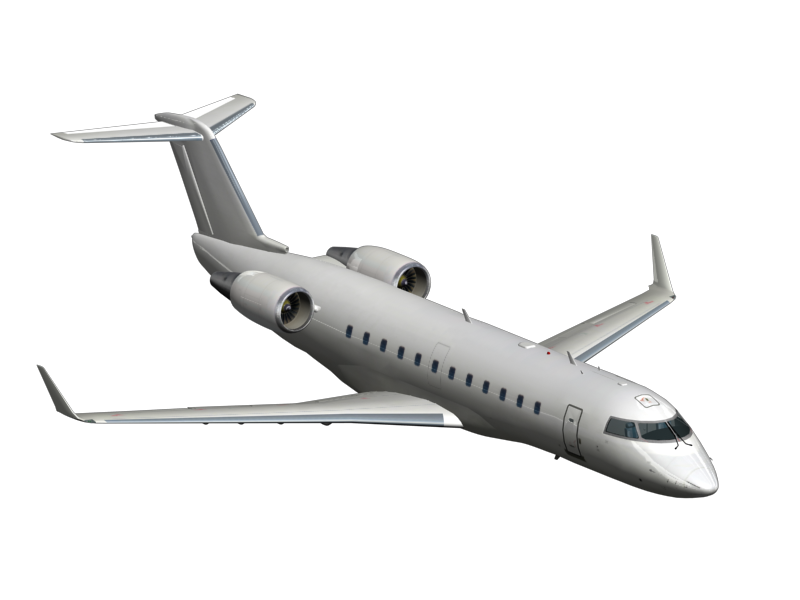
\includegraphics[width=0.49\linewidth]{Bombardier_CRJ200.png}}
  \end{subfigmatrix}
  \caption{Some aircrafts.}
  \label{fig:aircrafts}
\end{figure}

Make reference to Figures \ref{fig:airbus1} and \ref{fig:aircrafts}.

By default, the supported file types are {\it .png,.pdf,.jpg,.mps,.jpeg,.PNG,.PDF,.JPG,.JPEG}.

See \url{http://mactex-wiki.tug.org/wiki/index.php/Graphics_inclusion} for adding support to other extensions.


% ----------------------------------------------------------------------
\subsubsection{Drawings}
\label{subsection:drawings}

Insert your subsection material and for instance a few drawings...

The schematic illustrated in Fig.~\ref{fig:algorithm} can represent some sort of algorithm.

\begin{figure}[!htb]
  \centering
  \scriptsize
%  \footnotesize 
%  \small
  \setlength{\unitlength}{0.9cm}
  \begin{picture}(8.5,6)
    \linethickness{0.3mm}

    \put(3,6){\vector(0,-1){1}}
    \put(3.5,5.4){$\bf \alpha$}
    \put(3,4.5){\oval(6,1){}}
    %\put(0,4){\framebox(6,1){}}
    \put(0.3,4.4){Grid Generation: \quad ${\bf x} = {\bf x}\left({\bf \alpha}\right)$}

    \put(3,4){\vector(0,-1){1}}
    \put(3.5,3.4){$\bf x$}
    \put(3,2.5){\oval(6,1){}}
    %\put(0,2){\framebox(6,1){}}
    \put(0.3,2.4){Flow Solver: \quad ${\cal R}\left({\bf x},{\bf q}\left({\bf x}\right)\right) = 0$}

    \put(6.0,2.5){\vector(1,0){1}}
    \put(6.4,3){$Y_1$}

    \put(3,2){\vector(0,-1){1}}
    \put(3.5,1.4){$\bf q$}
    \put(3,0.5){\oval(6,1){}}
    %\put(0,0){\framebox(6,1){}}
    \put(0.3,0.4){Structural Solver: \quad ${\cal M}\left({\bf x},{\bf q}\left({\bf x}\right)\right) = 0$}

    \put(6.0,0.5){\vector(1,0){1}}
    \put(6.4,1){$Y_2$}

    %\put(7.8,2.5){\oval(1.6,5){}}
    \put(7.0,0){\framebox(1.6,5){}}
    \put(7.1,2.5){Optimizer}
    \put(7.8,5){\line(0,1){1}}
    \put(7.8,6){\line(-1,0){4.8}}
  \end{picture}
  \caption{Schematic of some algorithm.}
  \label{fig:algorithm}
\end{figure}


% ----------------------------------------------------------------------
\subsection{Equations}
\label{subsection:equations}

Equations can be inserted in different ways.

The simplest way is in a separate line like this

\begin{equation}
  \frac{{\rm d} q_{ijk}}{{\rm d} t} + {\cal R}_{ijk}({\bf q}) = 0 \,.
\label{eq:ode}
\end{equation}

If the equation is to be embedded in the text. One can do it like this ${\partial {\cal R}}/{\partial {\bf q}}=0$.

It may also be split in different lines like this

\begin{eqnarray}
  {\rm Minimize}   && Y({\bf \alpha},{\bf q}({\bf \alpha}))            \nonumber           \\
  {\rm w.r.t.}     && {\bf \alpha} \,,                                 \label{eq:minimize} \\
  {\rm subject~to} && {\cal R}({\bf \alpha},{\bf q}({\bf \alpha})) = 0 \nonumber           \\
                   &&       C ({\bf \alpha},{\bf q}({\bf \alpha})) = 0 \,. \nonumber
\end{eqnarray}

It is also possible to use subequations. Equations~\ref{eq:continuity}, \ref{eq:momentum} and \ref{eq:energy} form the Naver--Stokes equations~\ref{eq:NavierStokes}.

\begin{subequations}
    \begin{equation}
    \frac{\partial \rho}{\partial t} + \frac{\partial}{\partial x_j}\left( \rho u_j \right) = 0 \,,
    \label{eq:continuity}
    \end{equation}
    \begin{equation}
    \frac{\partial}{\partial t}\left( \rho u_i \right) + \frac{\partial}{\partial x_j} \left( \rho u_i u_j + p \delta_{ij} - \tau_{ji} \right) = 0, \quad i=1,2,3 \,,
    \label{eq:momentum}
    \end{equation}
    \begin{equation}
        \frac{\partial}{\partial t}\left( \rho E \right) + \frac{\partial}{\partial x_j} \left( \rho E u_j + p u_j - u_i \tau_{ij} + q_j \right) = 0 \,.
    \label{eq:energy}
    \end{equation}
\label{eq:NavierStokes}%
\end{subequations}


% ----------------------------------------------------------------------
\subsection{Tables}
\label{section:tables}

Insert your subsection material and for instance a few tables...

Make sure all tables presented are referenced in the text!

Follow some guidelines when making tables:

\begin{itemize}
  \item Avoid vertical lines
  \item Avoid “boxing up” cells, usually 3 horizontal lines are enough: above, below, and after heading
  \item Avoid double horizontal lines
  \item Add enough space between rows
\end{itemize}

\begin{table}[!htb]
  \renewcommand{\arraystretch}{1.2} % more space between rows
  \centering
  \begin{tabular}{lccc}
    \toprule
    Model           & $C_L$ & $C_D$ & $C_{M y}$ \\
    \midrule
    Euler           & 0.083 & 0.021 & -0.110    \\
    Navier--Stokes  & 0.078 & 0.023 & -0.101    \\
    \bottomrule
  \end{tabular}
  \caption[Table caption shown in TOC.]{Table caption.}
  \label{tab:aeroCoeff}
\end{table}

Make reference to Table \ref{tab:aeroCoeff}.

Tables \ref{tab:memory} and \ref{tab:multipleColumns} are examples of tables with merging columns:

\begin{table}[!htb]
  \renewcommand{\arraystretch}{1.2} % more space between rows
  \centering
  \begin{tabular}[]{lrr}
    \toprule
                & \multicolumn{2}{c}{\underline{Virtual memory [MB]}} \\
                & Euler       & Navier--Stokes \\
    \midrule
      Wing only &  1,000      &    2,000       \\
      Aircraft  &  5,000      &   10,000       \\
      (ratio)   & $5.0\times$ & $5.0\times$    \\
    \bottomrule
  \end{tabular}
  \caption{Memory usage comparison (in MB).}
  \label{tab:memory}
\end{table}

\begin{table}[!htb]
  \centering
  \renewcommand{\arraystretch}{1.2} % more space between rows
  \begin{tabular}{@{}rrrrcrrr@{}} % remove space to the vertical edges @{}...@{}
    \toprule
      & \multicolumn{3}{c}{$w = 2$} & \phantom{abc} & \multicolumn{3}{c}{$w = 4$} \\
    \cmidrule{2-4}
    \cmidrule{6-8}
      & $t=0$ & $t=1$ & $t=2$ && $t=0$ & $t=1$ & $t=2$ \\
    \midrule
      $dir=1$
      \\
      $c$ &  0.07 &  0.16 &  0.29 &&  0.36 &  0.71 &   3.18 \\
      $c$ & -0.86 & 50.04 &  5.93 && -9.07 & 29.09 &  46.21 \\
      $c$ & 14.27 &-50.96 &-14.27 && 12.22 &-63.54 &-381.09 \\
      $dir=0$
      \\
      $c$ &  0.03 &  1.24 &  0.21 &&  0.35 & -0.27 &  2.14 \\
      $c$ &-17.90 &-37.11 &  8.85 &&-30.73 & -9.59 & -3.00 \\
      $c$ &105.55 & 23.11 &-94.73 &&100.24 & 41.27 &-25.73 \\
    \bottomrule
  \end{tabular}
  \caption{Another table caption.}
  \label{tab:multipleColumns}
\end{table}

An example with merging rows can be seen in Tab.\ref{tab:multipleRows}.

\begin{table}[!htb]
  \renewcommand{\arraystretch}{1.2} % more space between rows
  \centering
  \begin{tabular}{ccccc}
    \toprule
      \multirow{2}{*}{ABC} & \multicolumn{4}{c}{header} \\
      \cmidrule{2-5} & 1.1 & 2.2 & 3.3 & 4.4 \\
    \midrule
      \multirow{2}{*}{IJK} & \multicolumn{2}{c}{\multirow{2}{*}{group}} & 0.5 & 0.6 \\
      \cmidrule{4-5}       & \multicolumn{2}{c}{}                       & 0.7 & 1.2 \\
    \bottomrule
  \end{tabular}
  \caption{Yet another table caption.}
  \label{tab:multipleRows}
\end{table}

If the table has too many columns, it can be scaled to fit the text widht, as in Tab.\ref{tab:scale}.
\begin{table}[!htb]
  \renewcommand{\arraystretch}{1.2} % more space between rows
  \centering
  \resizebox*{\textwidth}{!}{%
    \begin{tabular}[]{lcccccccccc}
      \toprule
        Variable &  a  &  b  &  c  &  d  &  e  &  f  &  g  &  h  &  i  &  j  \\
      \midrule
        Test 1   &  10,000 &  20,000 &  30,000 &  40,000 &  50,000 &  60,000 &  70,000 &  80,000 &  90,000 & 100,000 \\
        Test 2   &  20,000 &  40,000 &  60,000 &  80,000 & 100,000 & 120,000 & 140,000 & 160,000 & 180,000 & 200,000 \\
      \bottomrule
    \end{tabular}
  }%
  \caption{Very wide table.}
  \label{tab:scale}%
\end{table}


% ----------------------------------------------------------------------
\subsection{Mixing}
\label{section:mixing}

If necessary, a figure and a table can be put side-by-side as in Fig.\ref{fig:side_by_side}

\begin{figure}[!htb]
  \begin{minipage}[b]{0.60\linewidth}
    \centering
    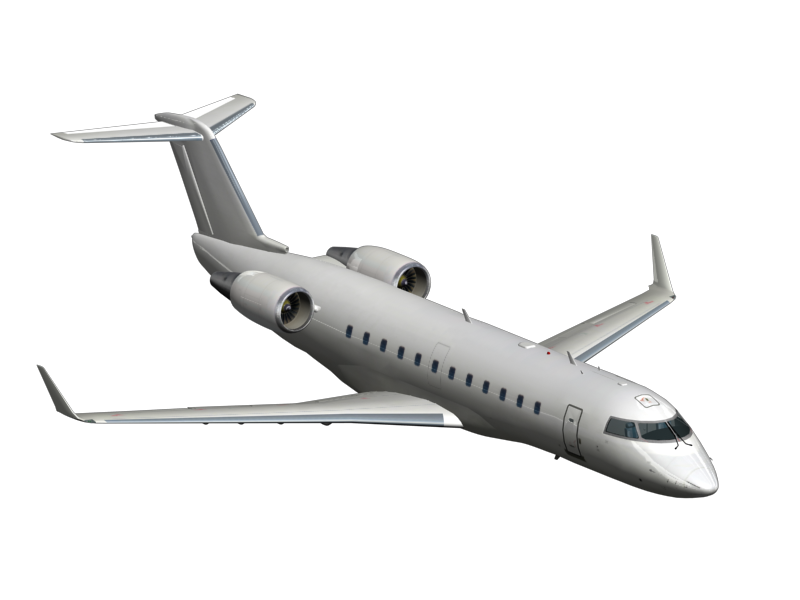
\includegraphics[width=\linewidth]{Bombardier_CRJ200}
  \end{minipage}%
  \begin{minipage}[b]{0.30\linewidth}
    \centering
    \begin{tabular}[b]{lll}
      \toprule
        \multicolumn{3}{c}{Legend} \\
      \midrule
        A & B & C \\
        0 & 0 & 0 \\
        0 & 1 & 0 \\
        1 & 0 & 0 \\
        1 & 1 & 1 \\
      \bottomrule
    \end{tabular}
    \vspace{5em}
  \end{minipage}
\caption{Figure and table side-by-side.}
\label{fig:side_by_side}
\end{figure}

 % file "Thesis_Results.tex"
\cleardoublepage

%%%%%%%%%%%%%%%%%%%%%%%%%%%%%%%%%%%%%%%%%%%%%%%%%%%%%%%%%%%%%%%%%%%%%%%%
%                                                                      %
%     File: Thesis_Conclusions.tex                                     %
%     Tex Master: Thesis.tex                                           %
%                                                                      %
%     Author: Andre C. Marta                                           %
%     Last modified :  2 Jul 2015                                      %
%                                                                      %
%%%%%%%%%%%%%%%%%%%%%%%%%%%%%%%%%%%%%%%%%%%%%%%%%%%%%%%%%%%%%%%%%%%%%%%%

\chapter{Conclusions}
\label{chapter:conclusions}

Insert your chapter material here...


% ----------------------------------------------------------------------
\section{Achievements}
\label{section:achievements}

The major achievements of the present work...


% ----------------------------------------------------------------------
\section{Future Work}
\label{section:future}

A few ideas for future work...

 % file "Thesis_Conclusions.tex"
\cleardoublepage

% ----------------------------------------------------------------------
%  Bibliography
% ----------------------------------------------------------------------

% Add entry in the table of contents as chapter
\phantomsection
\addcontentsline{toc}{chapter}{\bibname}

% Include all references in .bib file, even non-cited ones...
%\nocite{*} % this should be used carefully because it is not correct!

% Produces the bibliography section when processed by BibTeX
%
% Bibliography style
% > entries ordered alphabetically
%\bibliographystyle{plain}
% > unsorted with entries appearing in the order in which the citations appear.
%\bibliographystyle{unsrt}
% > entries ordered alphabetically, with first names and names of journals and months abbreviated
%\bibliographystyle{abbrv}
% > entries ordered alphabetically, with reference markers based on authors' initials and publication year
%\bibliographystyle{alpha}
%
% Replacement bibliography styles provided by 'natbib' package
% (plainnat.bst, abbrvnat.bst, unsrtnat.bst )
% > entries ordered alphabetically
%\bibliographystyle{plainnat}
% > unsorted with entries appearing in the order in which the citations appear.
%\bibliographystyle{unsrtnat}
% > entries ordered alphabetically, with first names and names of journals and months abbreviated
%\bibliographystyle{abbrvnat} % <<<<< SELECT IF USING REFERENCES BY AUTHOR/YEAR
% > entries ordered alphabetically, with reference markers based on authors' initials and publication year
%\bibliographystyle{alpha}
%
% Custom bibliography style adapted from 'natbib' package
%   (based on http://tex.stackexchange.com/questions/5053/is-it-possible-to-get-unsrt-abbrv-bibliography)
%   (unsrtnat.bst + abbrvnat.bst -> abbrvunsrtnat.bst)
%   (original files copied from:
%   http://tug.ctan.org/macros/latex/contrib/natbib/abbrvnat.bst
%   http://tug.ctan.org/macros/latex/contrib/natbib/unsrtnat.bst
% > unsorted with entries appearing in the order in which the citations appear, with first names and names of journals and months abbreviated.
\bibliographystyle{abbrvunsrtnat} % <<<<< SELECT IF USING REFERENCES BY NUMBER (CITATION ORDER)

% External bibliography database file in the BibTeX format
\bibliography{../Thesis_bib_DB} % file "Thesis_bib_DB.bib"

\cleardoublepage

% ----------------------------------------------------------------------
%  Appendix (optional)
%
%  CAUTION: 1) the main document (up to the conclusions) shall not exceed 80 pages
%           2) the document shall not exceed a total of 100 pages (per IST regulations)
% ----------------------------------------------------------------------
\appendix

% add page number prefix according to apendix chapter (optional)
%\renewcommand{\thepage}{\thechapter.\arabic{page}}

% re-set arabic numbering (A.1,A.2,...) (optional, use only if chapter prefix is added)
%\setcounter{page}{1}

%%%%%%%%%%%%%%%%%%%%%%%%%%%%%%%%%%%%%%%%%%%%%%%%%%%%%%%%%%%%%%%%%%%%%%%%
%                                                                      %
%     File: Thesis_Appendix_A.tex                                      %
%     Tex Master: Thesis.tex                                           %
%                                                                      %
%     Author: Andre C. Marta                                           %
%     Last modified :  2 Jul 2015                                      %
%                                                                      %
%%%%%%%%%%%%%%%%%%%%%%%%%%%%%%%%%%%%%%%%%%%%%%%%%%%%%%%%%%%%%%%%%%%%%%%%

\chapter{Vector calculus}
\label{chapter:appendixVectors}

In case an appendix if deemed necessary, the document cannot exceed a total of 100 pages...

Some definitions and vector identities are listed in the section below.

% ----------------------------------------------------------------------
\section{Vector identities}
\label{section:vectorIdentities}

\begin{equation}
	\nabla \times \left( \nabla \phi \right) = 0
	\label{eq:cross_nnp}
\end{equation}

\begin{equation}
	\nabla \cdot \left( \nabla \times {\bf u} \right) = 0
	\label{eq:dotCross_nnu}
\end{equation}



%%%%%%%%%%%%%%%%%%%%%%%%%%%%%%%%%%%%%%%%%%%%%%%%%%%%%%%%%%%%%%%%%%%%%%%%
\section{Theoretical Overview}
\label{section:overview}

Some overview of the underlying theory about the topic...


%%%%%%%%%%%%%%%%%%%%%%%%%%%%%%%%%%%%%%%%%%%%%%%%%%%%%%%%%%%%%%%%%%%%%%%%
\section{Theoretical Model 1}
\label{section:theory1}

The research should be supported with a comprehensive list of references.
These should appear whenever necessary, in the limit, from the first to the last chapter.

A reference can be cited in any of the following ways:
%
\begin{itemize}
  \item Citation mode \#1 - \quad \cite{jameson:adjointns}
  \item Citation mode \#2 - \quad \citet{jameson:adjointns}
  \item Citation mode \#3 - \quad \citep{jameson:adjointns}
  \item Citation mode \#4 - \quad \citet*{jameson:adjointns}
  \item Citation mode \#5 - \quad \citep*{jameson:adjointns}
  \item Citation mode \#6 - \quad \citealt{jameson:adjointns}
  \item Citation mode \#7 - \quad \citealp{jameson:adjointns}
  \item Citation mode \#8 - \quad \citeauthor{jameson:adjointns}
  \item Citation mode \#9 - \quad \citeyear{jameson:adjointns}
  \item Citation mode \#10 - \quad \citeyearpar{jameson:adjointns}
\end{itemize}
%
Several citations can be made simultaneously as \citep{nocedal:opt,marta:ijcfd}. \\

This is often the default bibliography style adopted (numbers following the citation order), according to the options:\\
{\tt \textbackslash usepackage\{natbib\}} in file {\tt Thesis\_Preamble.tex},\\
{\tt \textbackslash bibliographystyle\{abbrvnat\}} in file {\tt Thesis.tex}.\\
%
Notice however that this style can be changed from numerical citation order to authors' last name with the options: \\
{\tt \textbackslash usepackage[numbers]\{natbib\}} in file {\tt Thesis\_Preamble.tex},\\
{\tt \textbackslash bibliographystyle\{abbrvunsrtnat\}} in file {\tt Thesis.tex}.


%%%%%%%%%%%%%%%%%%%%%%%%%%%%%%%%%%%%%%%%%%%%%%%%%%%%%%%%%%%%%%%%%%%%%%%%
\section{Theoretical Model 2}
\label{section:theory2}

Other models...

 % file "Thesis_Appendix_A.tex"
\cleardoublepage

% re-set arabic numbering (B.1,B.2,...) (optional, use only if chapter prefix is added)
%\setcounter{page}{1}

%%%%%%%%%%%%%%%%%%%%%%%%%%%%%%%%%%%%%%%%%%%%%%%%%%%%%%%%%%%%%%%%%%%%%%%%
%                                                                      %
%     File: Thesis_Appendix_B.tex                                      %
%     Tex Master: Thesis.tex                                           %
%                                                                      %
%     Author: Andre C. Marta                                           %
%     Last modified :  2 Jul 2015                                      %
%                                                                      %
%%%%%%%%%%%%%%%%%%%%%%%%%%%%%%%%%%%%%%%%%%%%%%%%%%%%%%%%%%%%%%%%%%%%%%%%

\chapter{Technical Datasheets}
\label{chapter:appendixDatasheets}

It is possible to add PDF files to the document, such as technical sheets of some equipment used in the work.

% ----------------------------------------------------------------------
\section{Some Datasheet}
\label{section:datasheet}

% See more options to include PDF files in
% http://mirror.unl.edu/ctan/macros/latex/contrib/pdfpages/pdfpages.pdf
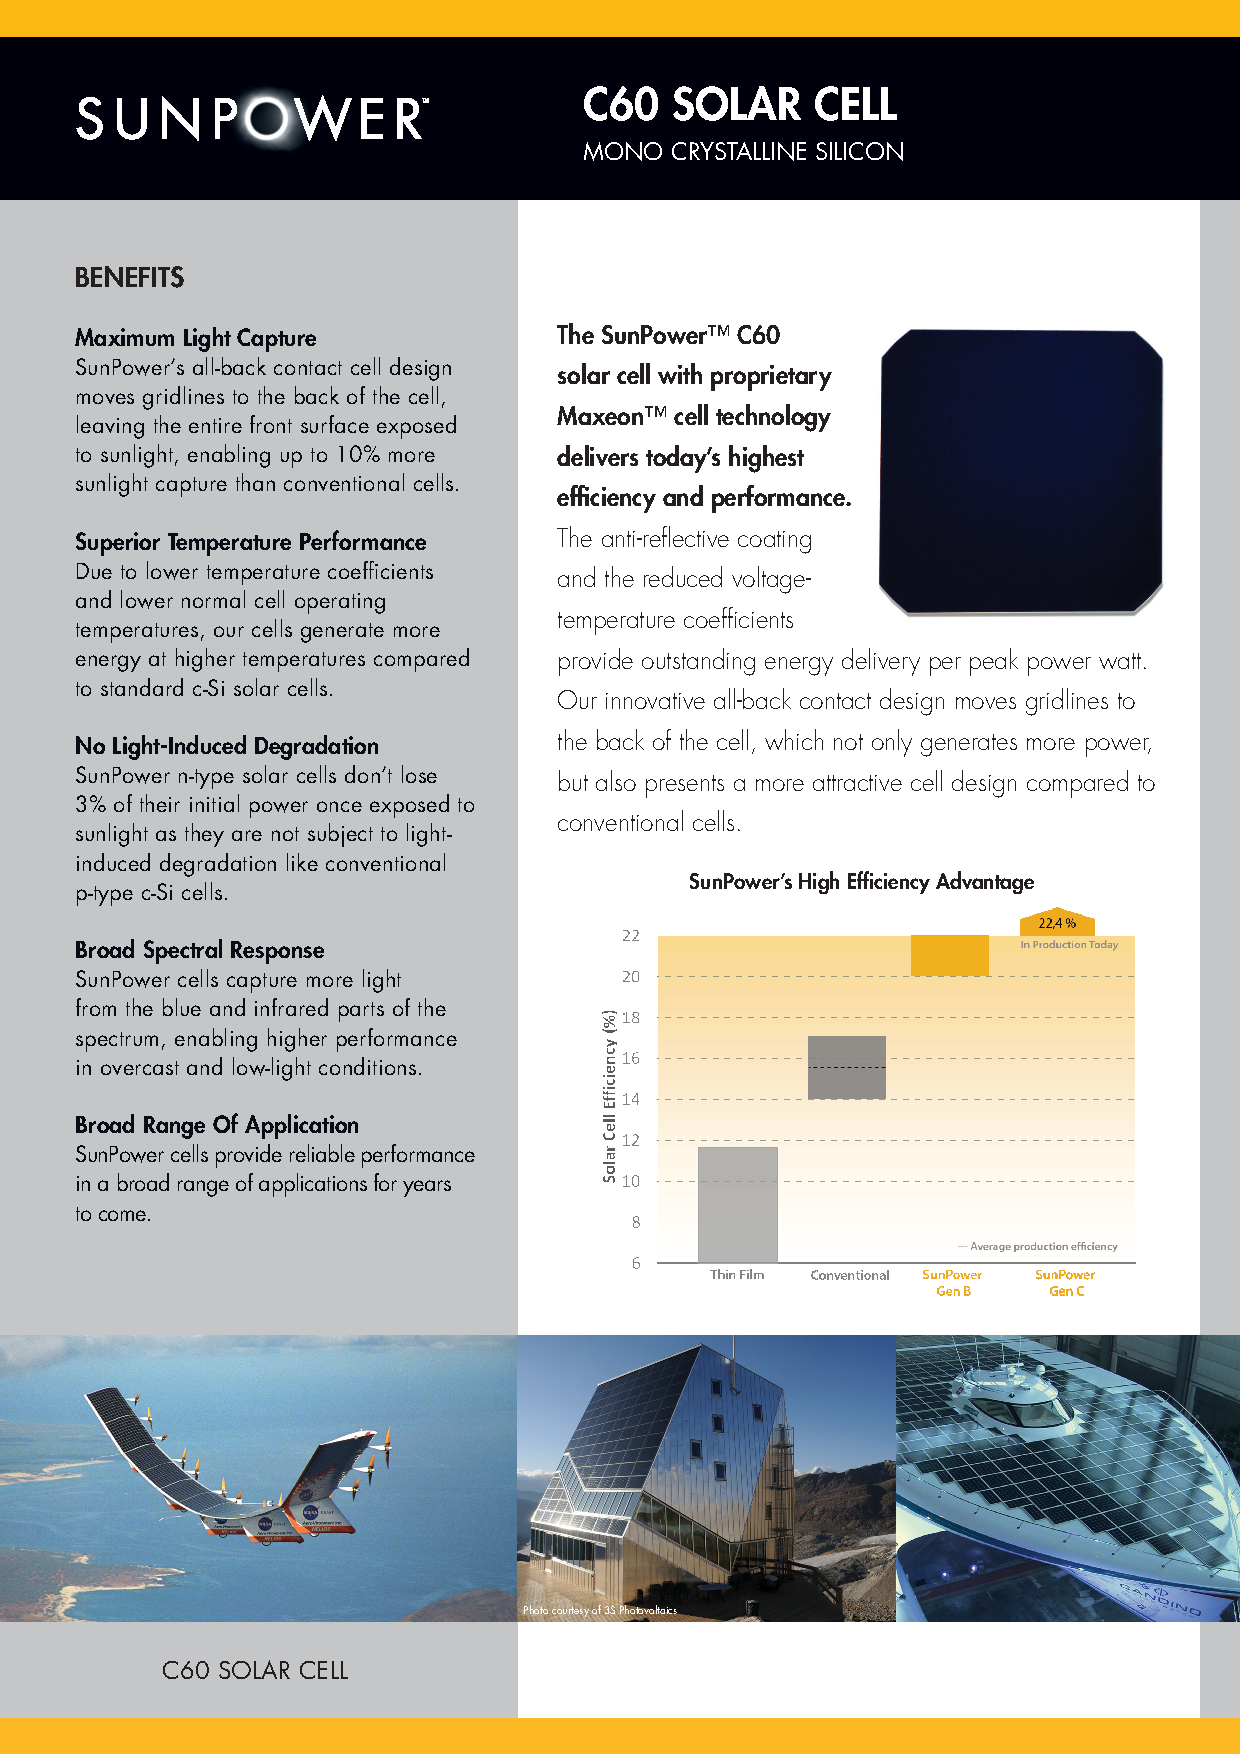
\includepdf[pages={1-2},nup=1x2,landscape=true]{SolarCell_Sunpower_C60.pdf}

 % file "Thesis_Appendix_B.tex"
\cleardoublepage

% ----------------------------------------------------------------------
\end{document}
% ----------------------------------------------------------------------